% Copyright (C) 2014-2020 by Thomas Auzinger <thomas@auzinger.name>

\documentclass[draft,final]{vutinfth} % Remove option 'final' to obtain debug information.

% Load packages to allow in- and output of non-ASCII characters.
\usepackage{lmodern}        % Use an extension of the original Computer Modern font to minimize the use of bitmapped letters.
\usepackage[T1]{fontenc}    % Determines font encoding of the output. Font packages have to be included before this line.
\usepackage[utf8]{inputenc} % Determines encoding of the input. All input files have to use UTF8 encoding.

% Extended LaTeX functionality is enables by including packages with \usepackage{...}.
\usepackage{amsmath}    % Extended typesetting of mathematical expression.
\usepackage{amssymb}    % Provides a multitude of mathematical symbols.
\usepackage{mathtools}  % Further extensions of mathematical typesetting.
\usepackage{microtype}  % Small-scale typographic enhancements.
\usepackage[inline]{enumitem} % User control over the layout of lists (itemize, enumerate, description).
\usepackage{multirow}   % Allows table elements to span several rows.
\usepackage{booktabs}   % Improves the typesettings of tables.
\usepackage{subcaption} % Allows the use of subfigures and enables their referencing.
\usepackage[ruled,linesnumbered,algochapter]{algorithm2e} % Enables the writing of pseudo code.
\usepackage[usenames,dvipsnames,table]{xcolor} % Allows the definition and use of colors. This package has to be included before tikz.
\usepackage{nag}       % Issues warnings when best practices in writing LaTeX documents are violated.
\usepackage{todonotes} % Provides tooltip-like todo notes.
\usepackage{hyperref}  % Enables cross linking in the electronic document version. This package has to be included second to last.
\usepackage[acronym,toc]{glossaries} % Enables the generation of glossaries and lists fo acronyms. This package has to be included last.
\usepackage{float}
% Copyright 2017 Sergei Tikhomirov, MIT License
% https://github.com/s-tikhomirov/solidity-latex-highlighting/

\usepackage{listings, xcolor}

\definecolor{verylightgray}{rgb}{.97,.97,.97}

\lstdefinelanguage{Solidity}{
	keywords=[1]{anonymous, assembly, assert, balance, break, call, callcode, case, catch, class, constant, continue, constructor, contract, debugger, default, delegatecall, delete, do, else, emit, event, experimental, export, external, false, finally, for, function, gas, if, implements, import, in, indexed, instanceof, interface, internal, is, length, library, log0, log1, log2, log3, log4, memory, modifier, new, payable, pragma, private, protected, public, pure, push, require, return, returns, revert, selfdestruct, send, solidity, storage, struct, suicide, super, switch, then, this, throw, transfer, true, try, typeof, using, value, view, while, with, addmod, ecrecover, keccak256, mulmod, ripemd160, sha256, sha3}, % generic keywords including crypto operations
	keywordstyle=[1]\color{blue}\bfseries,
	keywords=[2]{address, bool, byte, bytes, bytes1, bytes2, bytes3, bytes4, bytes5, bytes6, bytes7, bytes8, bytes9, bytes10, bytes11, bytes12, bytes13, bytes14, bytes15, bytes16, bytes17, bytes18, bytes19, bytes20, bytes21, bytes22, bytes23, bytes24, bytes25, bytes26, bytes27, bytes28, bytes29, bytes30, bytes31, bytes32, enum, int, int8, int16, int24, int32, int40, int48, int56, int64, int72, int80, int88, int96, int104, int112, int120, int128, int136, int144, int152, int160, int168, int176, int184, int192, int200, int208, int216, int224, int232, int240, int248, int256, mapping, string, uint, uint8, uint16, uint24, uint32, uint40, uint48, uint56, uint64, uint72, uint80, uint88, uint96, uint104, uint112, uint120, uint128, uint136, uint144, uint152, uint160, uint168, uint176, uint184, uint192, uint200, uint208, uint216, uint224, uint232, uint240, uint248, uint256, var, void, ether, finney, szabo, wei, days, hours, minutes, seconds, weeks, years},	% types; money and time units
	keywordstyle=[2]\color{teal}\bfseries,
	keywords=[3]{block, blockhash, coinbase, difficulty, gaslimit, number, timestamp, msg, data, gas, sender, sig, value, now, tx, gasprice, origin},	% environment variables
	keywordstyle=[3]\color{violet}\bfseries,
	identifierstyle=\color{black},
	sensitive=false,
	comment=[l]{//},
	morecomment=[s]{/*}{*/},
	commentstyle=\color{gray}\ttfamily,
	stringstyle=\color{red}\ttfamily,
	morestring=[b]',
	morestring=[b]"
}

\lstset{
	language=Solidity,
	backgroundcolor=\color{verylightgray},
	extendedchars=true,
	basicstyle=\footnotesize\ttfamily,
	showstringspaces=false,
	showspaces=false,
	numbers=left,
	numberstyle=\footnotesize,
	numbersep=9pt,
	tabsize=2,
	breaklines=true,
	showtabs=false,
	captionpos=b
}
\usepackage{seqsplit}
\newcommand{\hash}[1]{{\ttfamily\seqsplit{#1}}}
% Define convenience functions to use the author name and the thesis title in the PDF document properties.
\newcommand{\authorname}{Michael Etschbacher} % The author name without titles.
\newcommand{\thesistitle}{Reducing the operation cost of a file fixity storage service on the ethereum blockchain by utilizing pool testing strategies.} % The title of the thesis. The English version should be used, if it exists.
% Set PDF document properties
\hypersetup{
    pdfpagelayout   = TwoPageRight,           % How the document is shown in PDF viewers (optional).
    linkbordercolor = {Melon},                % The color of the borders of boxes around crosslinks (optional).
    pdfauthor       = {\authorname},          % The author's name in the document properties (optional).
    pdftitle        = {\thesistitle},         % The document's title in the document properties (optional).
    pdfsubject      = {Subject},              % The document's subject in the document properties (optional).
    pdfkeywords     = {a, list, of, keywords} % The document's keywords in the document properties (optional).
}

\setpnumwidth{2.5em}        % Avoid overfull hboxes in the table of contents (see memoir manual).
\setsecnumdepth{subsection} % Enumerate subsections.

\nonzeroparskip             % Create space between paragraphs (optional).
\setlength{\parindent}{0pt} % Remove paragraph identation (optional).

\makeindex      % Use an optional index.
\makeglossaries % Use an optional glossary.
%\glstocfalse   % Remove the glossaries from the table of contents.

% Set persons with 4 arguments:
%  {title before name}{name}{title after name}{gender}
%  where both titles are optional (i.e. can be given as empty brackets {}).
\setauthor{Bsc.}{\authorname}{}{male}
\setadvisor{Ao.univ.Prof. Dr.}{Andreas Rauber}{}{male}

% Required data.
\setregnumber{51828999}
\setdate{19}{05}{2022} % Set date with 3 arguments: {day}{month}{year}.
\settitle{\thesistitle}{\thesistitle} % Sets English and German version of the title (both can be English or German). If your title contains commas, enclose it with additional curvy brackets (i.e., {{your title}}) or define it as a macro as done with \thesistitle.

\setthesis{master}
\setthesis{master}
\setmasterdegree{dipl.} % dipl. / rer.nat. / rer.soc.oec. / master
\setcurriculum{Data Science}{Data Science} % Sets the English and German name of the curriculum.

\begin{document}

\frontmatter % Switches to roman numbering.
% The structure of the thesis has to conform to the guidelines at
%  https://informatics.tuwien.ac.at/study-services

\addtitlepage{naustrian} % German title page (not for dissertations at the PhD School).
\addtitlepage{english} % English title page.
\addstatementpage

\begin{danksagung*}
\todo{Ihr Text hier.}
\end{danksagung*}

\begin{acknowledgements*}
\todo{Enter your text here.}
\end{acknowledgements*}

\begin{kurzfassung}
\todo{Ihr Text hier.}
\end{kurzfassung}

\begin{abstract}
\todo{Enter your text here.}
\end{abstract}

% Select the language of the thesis, e.g., english or naustrian.
\selectlanguage{english}

% Add a table of contents (toc).
\tableofcontents % Starred version, i.e., \tableofcontents*, removes the self-entry.

% Switch to arabic numbering and start the enumeration of chapters in the table of content.
\mainmatter
\newacronym{eth}{ETH}{Ether}
\newacronym{p}{p}{Prevalence of corruption}
\newacronym{k}{k}{Optimal Pool Size}
\newacronym{oais}{OAIS}{Open Archival Information System}
\newacronym{eff}{E(S)}{Efficiency of strategy S compared to individual testing}
\newacronym{cost}{C(S)}{Cost Efficiency of strategy S compared to individual testing}
\newacronym{count_op}{T(S)}{Number of operations needed with strategy S}
\newacronym{count_wr}{TC(S)}{Number of cost relevant operations needed with strategy S}
\newacronym{individual}{$S_{i}$}{Individual testing strategy}
\newacronym{two-stage}{$S_{h}$}{Two-stage-hierarchical pooling strategy}
\newacronym{cs}{$S_{cs}$}{context-sensitive pooling strategy}
\newacronym{evm}{EVM}{Ethereum Virtual Machine}

\newglossaryentry{transaction}
{
  name={transaction},
  description={An Ethereum transaction refers to an action initiated by an account managed from a human, changes the state of the blockchain.}
}
\newglossaryentry{call}
{
  name={call},
  description={An Ethereum call refers to an interaction with a smart contract which does not change the state on the blockchain.}
}
\newglossaryentry{data-scrubbing}
{
  name={data-scrubbing},
  description={Data-scrubbing is an error correction technique which replaces corrupted object with copies.}
}
\newglossaryentry{history-forgery}
{
  name={history-forgery},
  description={The creation of false artifacts.}
}
\chapter{Introduction}
\section{About Data Integrity}
Storing cultural heritage in digital archives offers malicious actors the possibility to manipulate the data and possibly forge history. Recent digital technologies make data manipulation more efficient, less costly, and more exact and there is a long history of forging history. 
In 1920 a photography was taken of Vladimir Lenin atop a platform speaking to a crowd. In the original photo, see Figure \ref{fig:f1}, Lenin's comrade Leon Trotsky can be seen standing beside the platform on Lenin's left side. When power struggles within the revolution forced Trotsky out of the party 7 years later, he was retouched out of the picture, see Figure \ref{fig:f2}, using paint, razors and airbrushes. Soviet photo artists altered the historical record by literally removing Trotsky from the pictures \cite[3]{hofer2005digital}.

\begin{figure}[h]%
    \centering
    \begin{subfigure}{6cm}
    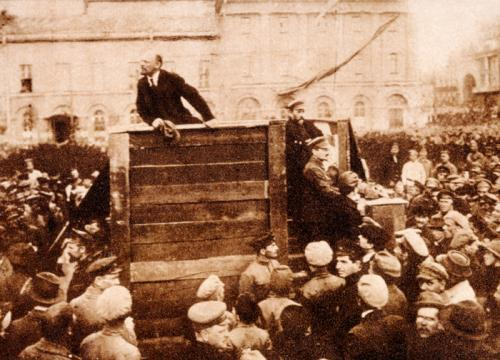
\includegraphics[width=\linewidth]{graphics/trotzki1.jpg}
    \caption{Original}\label{fig:f1}
    \end{subfigure}
    \qquad
    \begin{subfigure}{6cm}
    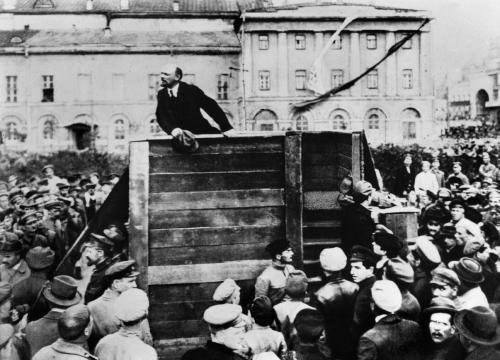
\includegraphics[width=\linewidth]{graphics/trotzki2.jpg}
    \caption{Original}
    \end{subfigure}
    \caption{Catalog Images}\label{fig:f2}
\end{figure}

Digital archives must earn the trust of current and future digital creators by developing a robust infrastructure and long-term preservation plans to demonstrate that the archive and its staff are trustworthy stewards of the digital materials in their care \cite[37]{kirschenbaum2010digital}. Digital objects can be corrupted easily, with or without fraudulent intent, and even without intent at all. Data corruption is usually detected by comparing cryptographic hashes, so-called fixity information, at different time intervals \cite[1]{de2014checking}. The object is seen as uncorrupted if the hash values are identical, since the smallest change to the object would alter the newly computed hash value immensely. 

\section{Research Problem}
Although generating fixity information (e.g., MD5, SHA-256) is relatively easy, managing that information over time is harder considering that if a malicious actor can alter the fixity information, the actor is also able to alter the underlying object illicit \cite[35]{kirschenbaum2010digital}. Fixity information is usually stored in databases; object metadata records or alongside content, whereas this thesis deals with blockchain as a storage medium. \cite{collomosse2018archangel} and \cite{Sigwart2020} have shown that the Ethereum blockchain, implemented by \cite{buterin2013ethereum}, can indeed be utilized to ensure data integrity, but there is a problem with that: the operation cost. The cost of storing a SHA256 values on the Ethereum blockchain is 20,000 gas (the unit for transaction fees), which oscillate at the time of writing at about \$5, which means the operation cost for an ingest of 10,000 objects costs about \$50,000.

\section{Research Goal}
This thesis proposes a way to reduce the operational cost of a blockchain-based fixity information storage by applying a pool testing strategy in which several digital objects are combined in a pool to form a hash list. The idea for this approach stems from the ongoing pandemic, in which the test capacities also must be used optimally.
\begin{quote}
Pool testing strategies build on testing a pooled sample from several patients: if the results from the pool test are negative, all patients in the pooled sample are declared not to have COVID-19; if the results of the pool are positive, each patient sample is tested individually. The pooled testing strategy is appealing, particularly when test availability is limited \cite[1]{cherif2020simulation}.
\end{quote}
This paradigm will be utilized in this thesis where the test specimen are cryptographic hashes, and the pool is hash list.

\section{Research Questions}
Based on the problem described above, the following research questions arise:

\textit{RQ1 What is the optimal pool size based on the corruption rates of digital objects in the archive in terms of efficiency and cost}

\textit{RQ2 To what extent can pooled object hashes increase the efficiency and reduce cost for a fixity information storage service on the Ethereum blockchain?}

\textit{RQ3 Given that metadata has a higher corruption rate, what effect has the split of metadata and objects on the operation cost?}

\section{Research Approach}
\label{sec:approach}
This work will follow the principles of Design Science Research, from \cite{hevner2007three}. The artifact is designed based on a literature review of the following main topics \textit{Diplomatics of Digital Records};\textit{Ethereum Blockchain}; and \textit{Pooled testing}.

The \textit{Application environment} is a digital archive which manages any kind of data, data will be referenced as information object in the archive and each object is provided with necessary metadata, as described in the OAIS reference model. I assume that the data integrity is ensured on ingest where a cryptographic hash value of the information object is computed and stored on the blockchain. The "location" of the fixity information on the blockchain is stored in the preservation description information in the form of a unique transaction hash, see Figure \ref{fig:oais-fixity}. 

\begin{figure}[h]
  \caption{The transaction hash, used to retrieve data from the blockchain, is stored in the fixity information of the PDI of an information object \cite[7]{lee2010open}}
  \label{fig:oais-fixity}
  \centering
    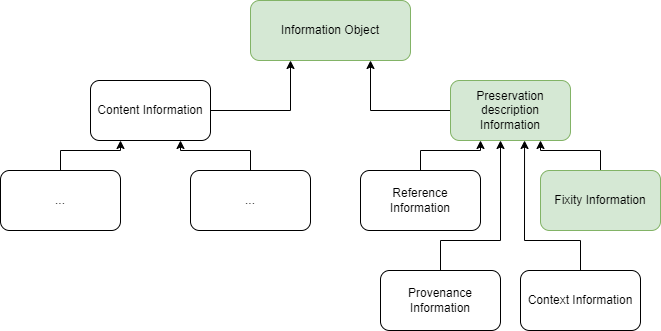
\includegraphics[width=0.7\textwidth]{oais.png}
\end{figure}

The \textit{Artifact} is a combination of decentralized application on the Ethereum blockchain and a local pool structure in the archive. The smart contract exposes functions for managing cryptographic hashes of pools.
The artifact must provide the following functionalities:
\begin{itemize}
  \item Create, Read, Update SHA256 values of pools.
  \item Must hold a reference (ID) for the respective pool in the archive.
  \item Must be tamperproof for unauthorized calls.
\end{itemize}
The smart contract complements the local pool structure in the archive where fixity information of certain object pools may be requested on any given time. The artifact should reduce the amount of operations needed to ensure the integrity of 10,000 objects from ingest to retrieval process by at least 50\%.
\chapter{Related Work}
The projects presented in this chapter are proposing various ways to utilize the Ethereum blockchain as a method to ensure the integrity of cultural heritage, sensor data or provenance data for the Internet of Things (IoT). The presented projects are related to my work in terms of design goals, where the immutability and decentralization of the Ethereum blockchain replaces trusted third parties. This chapter also gives an introduction to pooled testing and a state of the art method utilized in the medical field to test a large population on COVID-19.
\section{Project Archangel}
Project ARCHANGEL is a decentralized fixity information developed in the UK with the participation of three other countries, Australia, Estonia and Norway. Their approach is to store a cryptographic hash of every incoming object of the archive on a proof-of-authority blockchain. The project started in 2017 and ended in August 2018. The goal of the project was to ensure the integrity and authenticity of digital objects in archives with the usage a private fork of the Ethereum network. Their design philosophy of operating a private blockchain has the flaw of giving a few entities the power to alter data on the blockchain. Currently, their implementation uses smart contracts as a gateway for writing to the Blockchain \cite[4]{collomosse2018archangel}.

The public's trust in Archives and Memory Institutions (AMIs) has eroded, according to the authors of the project ARCHANGEL, due to the ease with which forgery and unauthorized modifications to electronic records can be carried out due to advances in technology and the creation of numerous types of composited content. Unlike in the past, when archives relied on specific firms' products and technologies, blockchain introduces a whole new paradigm of openness and expandability. The blockchain grants permission to write records in a distributed ledger to only authorized institutions, whereas permission to view the recorded content is granted to every node participating in the blockchain. Furthermore, scalability permits the use of diverse open-source tools and the assurance of record integrity by several parties through a consensus mechanism rather than by a single centralized organization. \cite[4]{wang2021research}.
The architecture of ARCHANGEL can be seen in Figure \ref{fig:archangel} where the cryptographic hash of an incoming object is computed and then persisted onto the private blockchain. After a certain time interval, the object can be retrieved from the archived and a hash will be recomputed with the same cryptographic hash function. The object is guaranteed to be unaltered if the local and online hash value are the same.
\begin{figure}[t]
    \centering
    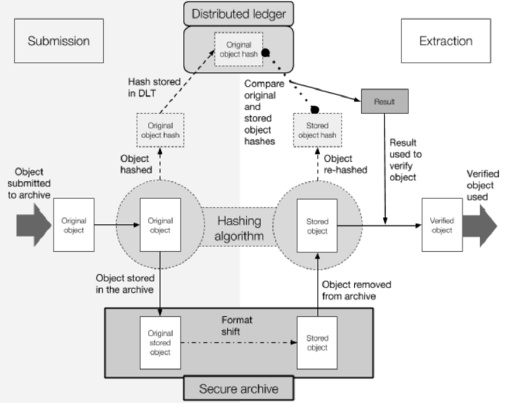
\includegraphics[width=0.5\textwidth]{archangel.png}
    \caption{Architecture of the ARCHANGEL platform \cite[2]{collomosse2018archangel}.}
    \label{fig:archangel}
\end{figure}
I agree with their vision of publicly available fixity information, where everyone with an Ethereum client is able to validate the integrity of objects in archive, but there are two points which do not conform with my vision. First and foremost is the usage of a private fork of the Ethereum network that is operated by a private set of nodes, which is basically a proof-of-authority consensus mechanism and contradicts the vision of a decentralized application \cite[3]{collomosse2018archangel}. Second, their implementation can hardly be used on the public Ethereum blockchain instead of a private fork due to the high cost of persisting data on the Ethereum main net, which is about \$8 for a SHA256 value, see Section \ref{sec:tx-cost}. 

\section{Provenance framework for the Internet of Things}
Sigwart et al. (2020) presents a data provenance framework for the IoT. Their approach is to store provenance records as so-called non-fungible assets on the Ethereum blockchain. Their prototype implements the ERC721 standard, which defines an interface for non-fungible assets or tokens (NFTs) which can be transferred by any clients (e.g., sensors, wallets), leaving a trail of provenance records created by passing the data NFT from owner to owner \cite[7]{Sigwart2020}. 
This project is important for my thesis, because it shows that the Ethereum blockchain can be utilized as a secure storage for immutable metadata which complements processes outside the blockchain.
Contrary to their implementation, I decided to not utilize the ERC721 standard since the data in my case, fixity information, does not need to be transferred from owner to owner. In order to use their implementation for fixity information instead of provenance data, you would have to deploy or "mint" an NFT for each digital object in the archive. That means, massive overhead in operation cost since "minting" is basically a deployment of a smart contract, which is one of the most expensive operations on the Ethereum blockchain, see Table \ref{table:gas-costs}.

\section{Remote Data Integrity Checking Scheme}
Zhao et al. (2020) presents a blockchain based remote data integrity checking scheme. Their scheme consists of three phases, including setup, storage and verification phase. This scheme may be of great importance for my work because it integrates well with the work of Sigwart et al. (2020) in terms of design goals. The detail of each phase in their scheme is described as follows: (1) Setup phase, where the public key is uploaded to the blockchain. (2) Storage phase, where the data owner signs the data blocks and uploads them to a cloud storage. (3) Verification phase, where the data owner downloads the data or desires to check the integrity of the individual data. The auditing process is done by verifying the signature of the data blocks by the data owner \cite[1]{zhao2020blockchain}.
The remote data integrity checking scheme utilizes the blockchain as a method to validate the integrity of IoT information management systems without involving trusted third parties, whereas the projects presented before utilizes the blockchain as a metadata storage.


\section{Pooled testing}\label{sec:pooled}
Pooled Testing was first introduced by \cite{dorfman1943detection} as a strategy to screen numerous military recruits for syphilis during World War 2. Dorfman envisioned that instead of testing each recruit's blood specimen separately, multiple specimens could be pooled together and tested at once. Positive pools' specimens would be retested individually to determine which recruits had contracted the disease, whereas negative pools' specimens would be declared negative. Dorfman wanted to save money on testing while still identifying all syphilitic-positive candidates, so he used group testing. Because the goal is to identify all positive persons among all individuals tested, this is now known as the "case identification problem." Dorfman's case identification method can be thought of as a two-stage hierarchical algorithm. Individuals from positive pools are tested in the second stage after non-overlapping pools have been screened in the first.

In this thesis, two strategies of pooled testing are implemented. 
First, two stage hierarchical pooling strategy, where in the first stage of this protocol N pools get initialized and filled with samples of the population. If the combined result of the pool is negative than no second stage is needed, but when a pool is declared positive a second stage is needed and all individuals from this pool have to be retested in order to find the corrupted individual. The expected number of test is equal to the number of tests in the first stage added to the number of tests in the second stage \cite[3]{nianogo2021optimal}.
The second strategy is context-sensitive pooling, where homogeneous samples are grouped in order to separate groups with different change rates. Hence, if one member of a pooled group is corrupted, there is a high likelihood that other group members are also corrupted \cite[3]{deckert2020simulation}.

\section{Summary}
The blockchain related projects presented in this chapter have a common vision, which is a decentralized storage for metadata to validate the integrity and authenticity of data used in applications. The ability for the public to validate that an authority did not tamper with the data in their care is important and the removal of trust strengthens the trust in public institutions. More on the subject of trust can be seen in Chapter \ref{ch:diplomatics}
Decentralization and trust aside, the cost of the fixity storage presented in this thesis is also more than relevant as later seen in Chapter \ref{ch:ethereum}, where the cost and computational effort of interacting with the Ethereum network is presented.

\chapter{Diplomatics of Digital Records}
\label{ch:diplomatics}
\section{About Diplomatics}
Diplomatics is a science that was developed in iplomatics is a science that was developed in France in the seventeenth century by the Benedictine
monk Dom Jean Mabillon in a treatise Diplomatics is a science that was developed in France in the seventeenth century by the Benedictine monk Dom Jean Mabillon in a treatise entitled De Re Diplomatica Libri VI (1681) for the purpose of ascertaining the provenance and authenticity of records
that attested to patrimonial rights. It later grewinto a legal, historical, and philological discipline as itcame to be used by lawyers to resolve disputes, by historians to interpret records, and by editors to publish medieval deeds and charters. It is useful to distinguish classic diplomatics from modern/digital diplomatics, because these two branches of the discipline do not represent a natural evolution of the latter from the former, but exist in parallel and focus on different objects of study. Modern diplomatics has a broader scope; it is concerned with all documents that are created in the course of affairs of any kind, and is define as “the discipline which studies the genesis, forms, and transmission” of records, and “their relationship with the facts represented in them and with their creator, in order to identify, evaluate, and communicate their true nature”. The primary focus of both classic and modern diplomatics is to assess the trustworthiness of records; however, the former establishes it retrospectively, looking at records issued several centuries ago, while the latter is concerned not only with establishing the trustworthiness of existing records but also with ensuring the trustworthiness of records that have yet to be created. \cite[10]{kirschenbaum2010digital}. 

Digital diplomatics defines a digital record as a digital component, or group of digital components, that is saved, and treated and managed as a record, or, more specifically, a record whose content and form are encoded using discrete numeric values, such as the binary values 0 and 1, rather than a continuous spectrum of values. A digital record is distinguished from an analogue record and an electronic record. InterPARES considers analogue the representation of an object or physical process through the use of continuously variable electronic signals or mechanical patterns. In contrast to a digitally encoded representa tion of an object or physical process, an analogue representation resembles the original. InterPARES defines an electronic record as any analogue or digital record that is carried by an electrical conductor and requires the use of electronic equipment to be intelligible by a person. InterPARES defines a record, using the traditional archival concept, as a document made or received in the course of a practical activity as an instrument or a by-prod uct of such activity, and set aside for action or reference \cite[52]{duranti2009digital}.

The integrity of a record is inferred not only from its appearance – which might be deceiving in the case of good forgeries – but also from the circumstances of its maintenance and preservation: an unbroken chain of responsible and legitimate custody is considered an insurance of integrity until proof to the contrary, and integrity metadata are required to attest to that. The authenticity of a record is a movable responsibility, as it shifts from the creators trusted recordkeeper, who needs to guarantee it for as long as the record is in its custody, to the trusted custodian, who guarantees it for as long as the record exists. \cite[53]{duranti2009digital}. In my thesis the Ethereum network acts as a trusted custodian which guarantees that no one is able to tamper with the cryptographic hash values of digital records.

\section{Trustworthiness}
Trustworthiness is a concept and an obligation that spans the life of a document, whether it is a sheaf of paper or a WordPerfect file. The needs of born-digital objects shift as files move through the stages of the preservation process, from initial capture and metadata extraction to longer-term strategies such as migration and rights management. Born-digital fonds are similarly mobile as they pass from the creator, to an intermediary such as a dealer or other agent (human or technological), to staff at an archival repository, and, finally, to storage and, perhaps, ingest into a digital repository. The stages of that journey constitute the chain of custody for a digital object, and each stage has important implications for the trustworthiness of the born-digital materials in a given accession. Authentic source may be deceptive or unreliable, and although reliability is an important component of trustworthiness, the veracity of a documents content is often not the concern of archivists working with cultural heritage materials. Rather, the provenance of both analog and digital materials, as well as documentation about their storage environment, what has been done to them, and by whom, are the key aspects of establishing and maintaining trust. Trustworthiness— of an institution, a custodian, or a document—plays an important role in the acquisition and maintenance of born-digital materials. How best to determine and document that quality in a digital environment and with regard to the stewardship of born-digital materials is a question that remains under consideration \cite[27]{kirschenbaum2010digital}. 

Digital diplomatics concerns itself with five aspects of trustworthiness: reliability, authenticity, accuracy, integrity and authentication \cite[10]{kirschenbaum2010digital}.

\subsection{Reliability}
Reliability is the trustworthiness of a record as a statement of fact, as to content. It is assessed on the basis of 1) the completeness of the record, that is, the presence of all the formal elements required by the juridical-administrative system for that specific record to be capable of achieving the purposes for which it was generated; and 2) the controls exercised on the process of creation of the record, among which are included those exercised on the author of the record, who must be the person competent, that is, having the authority and the capacity, to issue it. The reliability of a record is the exclusive responsibility of its creator and the trusted recordkeeper, that is, of the person or organization that made or received it and maintained it with its other records \cite[52]{duranti2009digital}.

The concept of reliability, used in reference to the source of the records, is defined in digital forensics in a way that points to a reliable software, measured by principles similar to those the courts use to determine evidentiary reliability, that is, empirical testing, subjection to peer review and publication, determination of error rate, and general acceptance within the relevant community. Also these principles point to open source software because the processes of records creation and maintenance can be authenticated with evidence either by describing a process or system used to produce a result, or by showing that the process or system produces an accurate result \cite[59]{duranti2009digital}.

\subsection{Authenticity}
Authenticity is the trustworthiness of a record as a record, and is defined as the fact that a record has not been tampered with or corrupted, either accident ally or maliciously. An authentic record is one that preserves the same identity it had when first generated, and can be presumed or proven to have maintained its integrity over time. The identity of a record is constituted of the whole of those characteristics that distinguish it from any other record, and is assessed on the basis of the formal elements on the face of the record, and/or its attributes, as expressed for example in a register entry or as metadata \cite[52]{duranti2009digital}.

The expectations of scholars with regard to the reliability of sources have evolved over the centuries, from the assumption that librarians and archivists would present researchers with evidence that could be relied upon to be verifiable, to more modern understandings that dispense with the ideal of the reliable source and consider all texts as potentially deceptive and richly ambiguous. Ideally, the methods of operation and processes developed by repositories over years of working with scholars and other patrons enable staff to provide researchers with documentation about the provenance and acquisition of the items in their care \cite[32]{kirschenbaum2010digital}.

\subsection{Accuracy}
Authenticity is the trustworthiness of a record as a record, and is defined as the fact that a record has not been tampered with or corrupted, either accident ally or maliciously. An authentic record is one that preserves the same identity it had when first generated, and can be presumed or proven to have maintained its integrity over time. The identity of a record is constituted of the whole of those characteristics that distinguish it from any other record, and is assessed on the basis of the formal elements on the face of the record, and/or its attributes, as expressed for example in a register entry or as metadata \cite[52]{duranti2009digital}.

\subsection{Integrity}
In the digital environment, there are no originals in the diplomatics sense, that is, there are no records which, in addition to being complete and capable of reaching the purposes for which they were generated (i.e., effective) are also the first instance of each item under consideration, because when we close a digital record for the first time we destroy the original and every time we open it we create a copy. However, we can state that each digital record, in the last version used by the creator in the usual and ordinary course of business, is a copy in the form of original and, in any version kept by the preserver, is an authentic copy of the record of the creator. They are both authoritative and authentic if their iden tity is intact and their integrity can be either presumed or proven. When extrating digital evidence, digital forensics must, first of all, avoid altering the data, and are guaranteed reliable in such sense by ensur ing that they are repeatable. Repeatability, which is one of the fundamental precepts of digital forensics practice, is supported by the accurate documentation of each and every action carried out on the evidence \cite[58]{duranti2009digital}. Such a chain of alteration is possible on the Ethereum network, since each update on an objects hash is natively documented on the blockchain.
Duplication integrity is ensured when given a data set, the process of creating a duplicate of the data does not modify the data (either intentionally or accidentally) and the duplicate is an exact bit copy of the original data set. It is possible to preserve data integrity over the duplicate, with respect to the original, by using a trusted third party. At the time the image is created, a copy of the hash can be given to a trusted third party to hold in escrow. Now changes to the duplicate can be detected even if the original is modified.
Digital forensics experts also link duplication integrity to time and have considered the use of time stamps for that purpose.63 A distinction between the integrity of a record as such and that of its duplicate may be useful to eliminate the conflict between the view of integrity held by diplomatists and that held by information technology experts, who tend to support the need for the extreme authentication provided by a digital signature. Indeed, one could further enrich the concept of integrity by also adopting the link between integrity and time proposed by digital forensics experts, and define record integrity differently in each phase of the record life cycle and/or custodial history \cite[60]{duranti2009digital}.
Both diplomatics and forensics were developed as practices for the purpose of investigating existing material evidence, assessing its status of transmission, its authenticity, and its ability to provide proof of facts at issue \cite[64]{duranti2009digital}.

\subsection{Authentication}
Authentication is defined as a declaration of authenticity made by a competent officer, and consists of a statement or an element, such as a seal, a stamp, or a symbol, added to the record after its completion. While authenticity is a quality of the record that accompanies it for as long as it exists as is, authentication only guarantees that a record is authentic at one specific moment in time, when the declaration is made or the authenticating element or entity is affixed. In the digital environment, extreme authentication is usually provided by a  igital signature. The digital signature has the function of a seal because it is attached to a complete record, allows verification of the origin and integrity of the record, and makes the record indisputable and incontestable by performing a non-repudiation function \cite[53]{duranti2009digital}.

\chapter{Ethereum Blockchain}
\label{ch:ethereum}
\section{Ethereum Blockchain}
\label{sec:eth-blockchain}
Open source blockchain networks such as Ethereum and Bitcoin are kits that allow you to set up an economic system in software, complete with account management, a native unit of exchange to pass between account. These native units of exchange are called coins, tokens, or cryptocurrencies, but the are no different from tokens in any other system: they are a form of money  that is usable only within that system to simply pay your peers or to run programs on the Ethereum network. When you want to make one of these peer-to-peer networks accessible through a web browser, you need to use special software libraries such as Web3.py (used in this thesis)\footnote{\url{https://github.com/ethereum/web3.py}} to connect an applications front end (the GUI you see in a browser), via JavaScript APIs, to its back end (the blockchain) \cite[2]{dannen2017introducing}.
The fact that everyone in the world can interact with the same distributed database, given you have internet access and a decent device, is favoritable in the case of an fixity storage as presented in \ref{chapter:fixity_storage} since anyone will be able to confirm if an object has changed over time. Lets say an digital archive releases multiple objects to the public and their respective fixity information on the blockchain, citizens could then validate if the object in question is really what it is meant to be. Trust in the archive is therefore not needed anymore, which will strenghten the general trust of the archive.
A block is a unit of time that encompasses a certain number of transactions. Inside that period, transaction data is recorded; when the unit of time elapses, the next block begins. The blockchain represents the history of state changes within the network database of the EVM \cite[43]{dannen2017introducing}.
Transactions and state changes in the Ethereum network are segmented into blocks, and then hashed. Each block is verified and validated before the next canonical block can be placed on top of it. In this way, nodes on the network do not need to individually evaluate the trustworthiness of every single block in the history of the Ethereum network, simply to compute the present balances of the accounts on the network. They merely verify that its “parent block” is the most recent canonical block. They do this quickly by looking to see that the new block contains the correct hash of its parents transactions and state. All the blocks strung together, and including the genesis block, an honorific describing the first block the network mined after coming online, are called the blockchain. In some circles, you will hear the blockchain referred to as a distributed ledger or distributed ledger technology (DLT). Ledger is an accurate description, as the chain contains every transaction in the history of the network, making it effectively a giant, balanced book of accounts \cite[55]{dannen2017introducing}. 
\section{Ethereum Virtual Machine}
\label{sec:evm}
The EVMs physical instantiation can not be described in the same way that one might point to a cloud or an ocean wave, but it does exist as one single entity maintained by thousands of connected computers running an Ethereum client \footnote{\url{https://ethereum.org/en/developers/docs/evm/}}.
A virtual machine (VM), in the Ethereum context, is one giant global computer composed of constituent nodes, which are themselves computers too. Generally speaking, a virtual machine is an emulation of a computer system by another computer system. These emulations are based on the same computer architectures as the target of their emulation, but they are usually reproducing that architecture on different hardware than it may have been intended for. Virtual machines can be created with hardware, software, or both. In the case of Ethereum, it is both. Rather than securely network thousands of discrete machines, Ethereum takes the approach of securely operating one very large state machine that can encompass the whole Earth \cite[48]{dannen2017introducing}.
The EVM can run arbitrary computer programs written in the Solidity\footnote{\url{https://github.com/ethereum/solidity}} language. These programs, given a particular input, will always produce the output the same way, with the same underlying state changes. This makes Solidity programs fully deterministic and guaranteed to execute, provided youve paid enough for the transaction. Solidity programs are capable of expressing all tasks accomplishable by computers, making them theoretically Turing complete. That means that the entire distributed network, every node, performs every program executed on the platform \cite[50]{dannen2017introducing}. 
From the perspective of a software developer, the EVM is also a runtime environment for small programs that can be executed by the network. The EVM has its own language, the EVM bytecode, to which your smart contracts compile. Solidity, which is a high-level language, is compiled into bytecode and uploaded onto the Ethereum blockchain by using a client application such as geth\footnote{\url{https://geth.ethereum.org/}} \cite[51]{dannen2017introducing}.
\section{Gas and Fees}
Gas refers to the unit that measures the amount of computational effort required to execute specific operations on the Ethereum network. Since each Ethereum transaction requires computational resources to execute, each transaction requires a fee. Gas refers to the fee required to conduct a transaction on Ethereum successfully.
Gas fees are paid in Ethereum's native currency, ether (ETH). Gas prices are denoted in gwei, which itself is a denomination of ETH - each gwei is equal to 0.000000001 ETH (10-9 ETH). For example, instead of saying that your gas costs 0.000000001 ether, you can say your gas costs 1 gwei. The word 'gwei' itself means 'giga-wei', and it is equal to 1,000,000,000 wei. Wei itself is the smallest unit of ETH\footnote{\url{https://ethereum.org/en/developers/docs/gas/}}.
\section{Smart Contracts}
Smart contracts are the building blocks of decentralized applications running on the EVM, they are like the concept of classes in conventional object-oriented programming. When developers speak of writing smart contracts, they are typically referring to the practice of writing code in the Solidity language to be executed on the Ethereum network. When the code is executed, units of value may be transferred as easily as data \cite[10]{dannen2017introducing}.
In my thesis, the fixity storage is often referenced as decentralized application (DAPP) which is built with several smart contracts. The main smart contract used in this thesis is further described in Section \ref{chapter:fixity_storage}. 

\section{Persistence}
Unlike a centralized server operated by a single company or organization, decentralized storage systems consist of a peer-to-peer network of user-operators who hold a portion of the overall data, creating a resilient file storage sharing system. These can be in a blockchain-based application or any peer-to-peer-based network. Ethereum itself can be used as a decentralized storage system, and it is when it comes to code storage in all the smart contracts. However, when it comes to large amounts of data, that isn't what Ethereum was designed for. The chain is steadily growing, but at the time of writing, the Ethereum chain is 602.95 GB for Mar 19 2022\footnote{\url{https://ycharts.com/indicators/ethereum_chain_full_sync_data_size}}, and every node on the network needs to be able to store all of the data. If the chain were to expand to large amounts of data (say 5TBs) it wouldn't be feasible for all nodes to continue to run. Also, the cost of deploying this much data to Mainnet would be prohibitively expensive due to gas fees \footnote{\url{https://ethereum.org/en/developers/docs/storage/}}.
My proposed solution using pooled testing, presented in Section \ref{chapter:pooled_testing}, counters the ever increasing chain size of the Ethereum network by reducing the amount of write transaction by at least 50 percent. Each writing transaction performed from the fixity storage stores exactly one sha256 result, on the blockchain. The gas cost of storing 256 bit on the blockchain can be read from Table \ref{table:gas-costs}.
All transactions in Ethereum are stored on the blockchain, a canonical history of state changes stored on every single Ethereum node \cite[12]{dannen2017introducing}.
Like all databases, a blockchain has a schema: rules define, constrain, and enforce relationships between entities. Motivations to break or alter these relationships can be found across industries, leading to bribery and corruption, and making blockchains trustless qualities even more attractive to business than prior generations of software and networking. In all databases, shared read/write access creates enormous complexity. Machines all over the world may experience varying latency, depending on where the database is physically located, leading to some write operations arriving out of order. This gets even more difficult if several parties are supposed to equally share a database \cite[20]{dannen2017introducing}. 
The nodes go through the block they are process and run any code enclosed within the transactions. Each node does this independently; it is not only highly parallelized, but highly redundant. Despite the high redundany, this is an efficient way to balance a global ledger in a trustworthy way \cite[50]{dannen2017introducing}.
\subsection{Blockchain-based persistence}
This type of persistence is utilized in my thesis, since the fixity information of the archived objects are meant to be persisted for longterm.
For a piece of data to persist forever, Ethereum needs to use a persistence mechanism. For example, on Ethereum, the persistence mechanism is that the whole chain needs to be accounted for when running a node. New pieces of data get tacked onto the end of the chain, and it continues to grow - requiring every node to replicate all the embedded data. This is known as blockchain-based persistence. The issue with blockchain-based persistence is that the chain could get far too big to upkeep and store all the data feasibly (e.g. many sources estimate the Internet to require over 40 Zetabytes of storage capacity). The blockchain must also have some type of incentive structure. For blockchain-based persistence, there is a payment made to the miner. When the data is added to the chain, the nodes are paid to add the data on \footnote{\url{https://ethereum.org/en/developers/docs/storage/}}.
\subsection{Contract-based persistence}
Contract-based persistence has the intuition that data cannot be replicated by every node and stored forever, and instead must be upkept with contract agreements. These are agreements made with multiple nodes that have promised to hold a piece of data for a period of time. They must be refunded or renewed whenever they run out to keep the data persisted. In most cases, instead of storing all data on-chain, the hash of where the data is located on a chain gets stored. This way, the entire chain doesn't need to scale to keep all of the data \footnote{\url{https://ethereum.org/en/developers/docs/storage/}}.
\section{Test Networks}. 
These networks are not really free of charge, but the ether token on the respective network is free to get. Although the queue of the free ether token can be very vast in some cases e.g. https://faucet.dimensions.network/ this faucet has a waiting queue for over three days until you recieve one ether token for the ropsten network. Other faucets, a distributer of free ether test tokens, require social network accounts to verifiy that you are not a bot e.g. https://faucet.paradigm.xyz/ requires a twitter account with at least one tweet and at least 15 retweets before you can request one ether token. The faucet request are almost all time gated, meaning that you could request ether only once per day. At small scale, this limitation is no problem for this thesis because persisting around 10 pools on the blockchains require at max 0.002 ether tokens. The one per day paradigm gets problemeatic for the experiment for the 10.000 objects, which costs about 20 ether tokens, which means I would have to request tokens fors 20 days straight to perform one experiment on a real live environment such as the ropsten testnetwork. 
There are multiple options to choose from for a testnetwork, from the most prominent networks presented at the official ethereum documentation https://ethereum.org/en/developers/docs/networks/ only the ropsten network implements the proof-of-work algorithm, which means it is the best representation of ethereum to date, and for that reason I decided to utilize the ropsten network in this experiment
\section{Costs}
\label{sec:costs}
Miners are paid this ether for mining, and also for running scripts on the network. The cost associated with electricity expenditure of servers running on the Ethereum network is one of the factors that gives ether, as a cryptocommodity, its intrinsic value—that is, someone paid real money to their electricity company to run their mining machine. Specialized mining rigs, which use arrays of graphics cards to increase their odds of completing a block and getting paid \cite[12]{dannen2017introducing}. 
Mining achieves the consensus required to make valid state changes, and the miners are paid for contributing to the consensus building. This is how ether and bitcoin are created  \cite[57]{dannen2017introducing}. 
For every instruction the EVM executes, there must be a cost associated, to ensure the system isnt jammed up by useless spam contracts. Every time an instruction executes, an internal counter keeps track of the fees incurred, which are charged to the user. Each time the user initiates a transaction, that users wallet reserves a small portion to pay these fees \cite[58]{dannen2017introducing}. The fees are the driving factor of my thesis where I try to make as less transactions as possible to run a fixity storage system on the Ethereum network. 
The fees are dependent on the gas cost of a transaction, gas is a unit of work; it is not a subcurrency, and you can not hold or hoard it. It simply measures how much effort each step of a transaction will be, in computational terms. To be able to pay for gas costs, you simply need to add ether to your account. You do not have to acquire it separately; there is no gas token. Every operation possible on the EVM has an associated gas cost. Gas costs ensure that computation time on the network is appropriately priced \cite[59]{dannen2017introducing}.
If you send a computationally difficult set of instructions to the EVM, the only person this hurts is you. The work will spend your ether, and stop when the ether you allocated to the transaction runs out. It has no effect on anyone elses transactions. There is no way to jam up the EVM without paying a lot, in the form of transaction fees, to do it. Scaling is handled in a de facto way through the gas fee system. Miners are free to choose the transactions that pay the highest fee rates, and can also choose the block gas limit collectively. The gas limit determines how much computation can happen (and how much storage can be allocated) per block \cite[60]{dannen2017introducing}. 
\section{Transactions}
An Ethereum transaction refers to an action initiated by an externally-owned account, in other words an account managed by a human, not a contract. For example, if Bob sends Alice 1 ETH, Bob's account must be debited and Alice's must be credited. This state-changing action takes place within a transaction. 
\begin{figure}[h]
    \caption{Illustration of an ethereum transaction \url{https://ethereum.org/en/developers/docs/transactions/}}
    \centering
    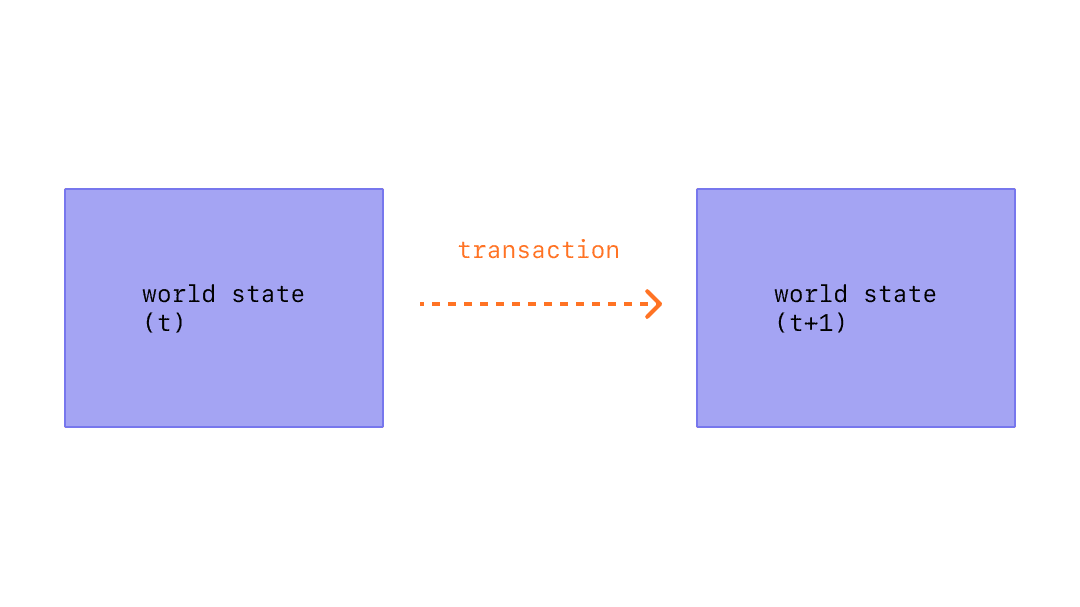
\includegraphics[width=0.5\textwidth]{eth_transaction.png}
\end{figure}
Transactions, which change the state of the EVM, need to be broadcast to the whole network. Any node can broadcast a request for a transaction to be executed on the EVM; after this happens, a miner will execute the transaction and propagate the resulting state change to the rest of the network. \footnote{\url{https://ethereum.org/en/developers/docs/transactions/}}.
\begin{verbatim}
{
  from: "0xAF8725604990d46042A50EfD9e2cB118141Bb140",
  to: "0x2C3c7752cE837bB97D6C31B4f883EAAA92BC3Ce5",
  gasLimit: "21000",
  maxFeePerGas: "300",
  maxPriorityFeePerGas: "10",
  nonce: "42",
  value: "10000000000"
}
\end{verbatim}
Transactions come from external accounts, which are usually controlled by human users. It is a way for an external account to submit instructions to the EVM to perform some operation. In other words, it is a way for an external account to get a message into the system. A transaction in the EVM is a cryptographically signed data package storing a message, which tells the EVM to transfer ether, create a new contract, trigger an existing one, or perform some calculation. Contract addresses can be the recipients of transactions, just like users with external accounts \cite[60]{dannen2017introducing}. 
Table \ref{table:gas-costs} presents the gas cost of the most used operation used in this thesis according to the Ethereum yellow paper \cite[27]{wood2014ethereum}.
\begin{center}
    \begin{tabular}{ c c c }\label{table:gas-costs}
     Operation Name & Gas Cost & Description \\ 
     $G_codedeposit$ & 200 & gas cost per bytesize of the compiled bytecode of the smart contract \\  
     $G_txcreate$ & 32000 & create a new smart contract  \\   
     $G_transaction$ & 21000 & retrieve the current balance of an account \\
     $G_txdatanonzero$ & 16 & gas cost per bytesize of the compiled bytecode of the transaction  \\   
     $G_balance$ & 400 & retrieve the current balance of an account 
    \end{tabular}
\end{center}
\section{Events}
\label{sec:events}
\chapter{Fixity Storage}
\label{ch:fixity_storage}
\section{Fixity Information}
Fixity Information provides the Data integrity checks or validation/verification keys used to ensure that the particular Content Information object has not been altered in an undocumented manner\cite[8]{lee2010open}. In this thesis, fixity information will be a transaction hash, with which the fixity information can be retrieved from the Ethereum blockchain.
With fixity information you are able to answer questions regarding the authenticity and integrity of an object, which supports assertions about the authenticity and trustworthiness of digital objects \cite[3]{ndsa2017fixity}.
\newline \textit{Have you received the files you expected?} When fixity information is provided with objects upfront, it can be used to validate that you have received what was intended for the collection.
\newline \textit{Is the data corrupted or altered from what you expected?}  Once you have generated baseline fixity information for files or objects, comparing that information with future fixity check information will tell you if a file has changed or been corrupted.
\newline \textit{Can you prove you have the data/files you expected, and they are not corrupt or altered?} By providing fixity information alongside content, you enable your users to verify that what they have is identical to what you say it should be. 

Fixity is a key concept for the long-term preservation and management of digital material for many reasons. Previous scholarship on fixity has shown its vital importance in discovering changes to data and all that this error-checking can imply: authenticity and renderability of files, trustworthiness of institutions, and system monitoring/maintenance. Despite the centrality of fixity to the field of digital preservation, there is little prescriptive guidance on when and how to create fixity information, where to store it, and how often to check it. This absence is not without reason, however: the incredible variety of organizational structures, priorities, staffing levels, funding, resources, and size of collections held by institutions that do digital preservation make it difficult to establish a single set of one-size-fits-all best practices \cite[38]{ndsa2017fixity}.
\subsection{Generating Fixity Information on Ingest}
 It is important to check the fixity
of content transferred to you when you bring it under your stewardship. Whenever possible, it is ideal to encourage content providers or producers to submit fixity information along with content objects. You can only provide assurance about the fixity of content overtime once you have initial fixity values, thus it is imperative to document fixity information as soon as possible. If fixity information is not provided as part of the transfer, you should create fixity information once you have received the materials \cite[4]{ndsa2014fixity}.

\subsection{Fixity Checks}
In addition to checking fixity before and after transfer, collections of digital files and objects should be checked on a regular basis. There are a range of systems and approaches focused on checking the fixity values of all objects at regular intervals. This could be monthly, quarterly, or yearly for example. The more often you check, the more likely you are to detect and repair errors \cite[4]{ndsa2014fixity}.
The information must be put to use, in the form of scheduled audits of the objects against the fixity information. Additionally, replacement or repair processes must be in place. Ideally these will have been tested before being needed. All of this is critical for bit-level preservation, but ensuring fixity does not mean that the object is or will be understandable. Long term access is also contingent on ones ability to make sense of and use the contents of the file in the future \cite[2]{ndsa2014fixity}.

Most fixity procedures involve a computational method that takes a digital file as input and outputs an alphanumeric value; this output value is used as a baseline comparison each time the fixity check is rerun \cite[5]{ndsa2017fixity}. 
For example, fixity checks may occur at different times depending on the institution's environment: during initial deposit only; during any file transmission; during scheduled backup routines; or periodically at specified times or when manually triggered \cite[7]{ndsa2017fixity}.\newline The rate of fixity checking is going to be dependent on how quickly you can run the checks, the complexity of your chosen fixity instrument, and how much of your resources (e.g., CPU, memory, bandwidth) can be used for this operation. This can become a choke point as the amount of digital content increases but the infrastructure to perform the checks stays the same. In a situation like this, the fixity checking activities can adversely affect other important functions like delivery of the content to users.
\subsection{Fixity Instruments}
\begin{table}[p]
    \centering
    \caption{Various Fixity Instruments \cite[6]{ndsa2017fixity}}
    \label{tb:fixity-instruments}
    \begin{tabular}{c|p{0.4\textwidth}|p{0.4\textwidth}}
     Fixity Instrument & Definition & Level of Effort and Return of Investment\\
     \hline
     Expected File Size & File size that differs from the expected can be an indicator of problems, for example by highlighting zero byte files & Low level of effort and low level detail. File size is auto-generated technical metadata that can be viewed in Windows Explorer or other common tools. \\  
     \hline
     Expected File Count & File count that differs from the expected can be an indicator that files are either added or dropped from the package. & Low level of effort and low level detail. File count is auto-generated technical metadata that can be viewed in Windows Explorer or other common tools.  \\
     \hline
     CRC & Error detection code, typically used during network transfers. & Low level of effort and moderate level of detail. CRC function values, which are variable but typically 32 or 64 bit, are relatively easy to implement and analyze.  \\
     \hline
     MD5 & Cryptographic hash function & Moderate level of effort and high level of detail. CPU and processing requirements to compute the hash values are low to moderate depending on the size of the file. The output size of this hash value is the lowest of the cryptographic hash values at 128 bits.  \\
     \hline
     SHA1 & Cryptographic hash function & Moderate level of effort, high level of detail, and added security assurance. Due to its higher 160-bit output hash value, SHA-1 requires more relative time to compute for a given number of processing cycles CPU and processing time than MD5.  \\
     \hline
     SHA256 & More secure cryptographic hash function & High level of effort, very high level of detail, and added security assurance. With an output hash value of 256 bits, SHA-256 requires more relative time to compute for a given number of processing cycles CPU and processing time than SHA-1. 
    \end{tabular}
\end{table}
For a given fixity instrument, see Table \ref{tb:fixity-instruments}, the harder it is to find two objects that result in the same fixity information, the more “collision resistant” that instrument is. This is important mostly for preventing the concealment of intentional changes to objects. For example, expected file size and expected file count are extremely vulnerable to collision: it is very easy for someone to replace an object with one that matches in file size. It is also possible (although unlikely) for an unintentional change (such as corruption or human error) to result in an object with the same fixity information for instruments that have low collision resistance. Of the fixity instruments described above, the cryptographic hash functions (MD-5, SHA-1, and SHA-256) are the most collision resistant; SHA-256 is recommended for applications where security is important. However, performing fixity checking and replacing damaged objects is critical for any preservation system, and using any fixity instrument is much better than none at all. Note that as the level of security of the hash function increases, so do the time and resources needed to compute \cite[7]{ndsa2014fixity}.
\subsection{Storage Medium}
\label{sec:storage-medium}
There are various storages to store fixity information, each of them has some advantages and disadvantages in terms of conveniency, security and throughput.
\newline \textit{In object metadata records:} In many cases, you will want to record some file or object fixity information wherever you store and manage the metadata records. These metadata records are actually stored as discrete files or in databases. This is particularly useful for maintaining originally submitted or generated fixity information as part of the long-term object metadata. 
\newline \textit{In databases and logs:} For checks you run at given intervals you may not want to be constantly adding to your object metadata records. In this case, it makes sense to keep running fixity information in databases and logs that you can return to when needed.
\newline \textit{Alongside content:} Its often ideal to have fixity information right alongside the content itself. That way, if you have problems with other layers in your system, or want to transfer some set of objects, you still have a record of previous fixity values alongside your content. For example, the BagIt specification includes a requirement for a hash value for the bagged content alongside the content. Similarly, some workflows involve creating *.md5 files, which are simply text files with the md5 hash, named identically to the file it refers to, but with an additional .md5 extension.
\newline \textit{In the files themselves:} When a checksum is for a portion of a file, it may make sense to store the information directly in the file. Note that this only makes sense when storing sub-file fixity information within a file. Adding fixity information for an entire file to the file itself changes the file and therefore changes its fixity value \cite[7]{ndsa2014fixity}.
\newline \textit{Ethereum Blockchain:} In this thesis I have chosen the blockchain to be the storage-medium for the fixity information. Its immutable state and availability in addition to its novel use-case in digital archives have influenced my decision.
\section{Example of a fixity storage}
A fixity storage must persist any kind of fixity information, in my thesis SHA256 values, for long term and guarantee that the persisted content is unaltered until retrieval of the content. I have chosen the Ethereum network as a medium for persisting file fixity information, see Section \ref{sec:storage-medium} for my reasoning. In Figure \ref{fig:lifecycle} the lifecycle of fixity information is presented, where at some point in time the information is ingested into the storage and after a certain time interval the information is fetched and compared to the retrieved SHA256 value from the digital object of the archive. If both cryptographic hashes match, the object is guaranteed to be unaltered. 
\begin{figure}[b]
  \caption{Example of a fixity storage}
  \label{fig:lifecycle}
  \centering
    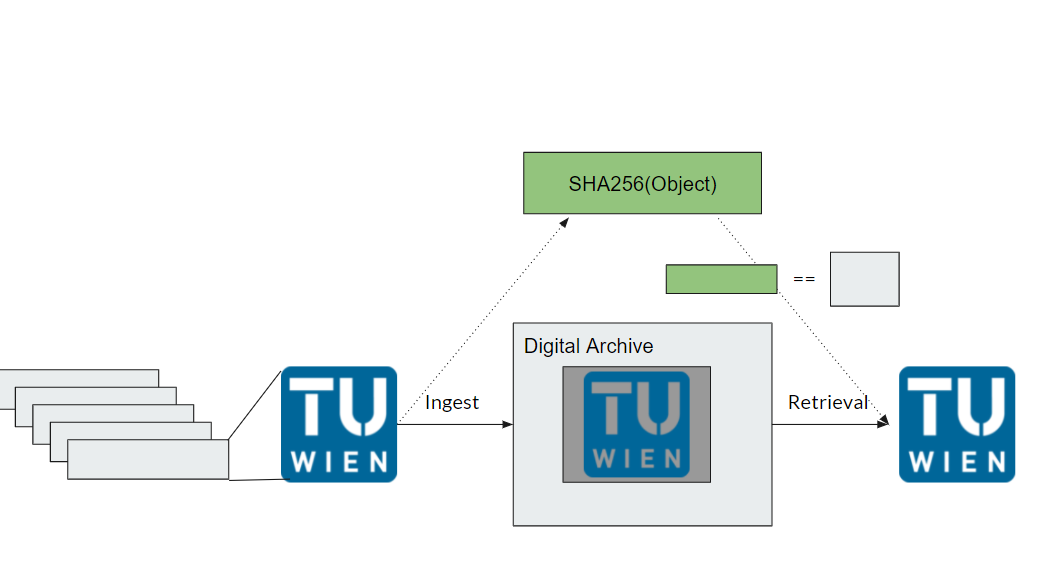
\includegraphics[width=0.75\textwidth]{lifecycle.png}
\end{figure}
\section{Implementation}
\label{sec:implementation}
The fixity storage presented in this thesis is implemented in Solidity, a programming language designed for the EVM, see Section \ref{sec:evm}.
The basic functionality of the smart contract, as described in Section \ref{sec:approach} can be seen in the source code presented in Listing \ref{lst:fixity-storage}
\begin{lstlisting}[language=Solidity,caption={MVP source code of the fixity storage deployed on the Ropsten test network \url{https://Ropsten.etherscan.io/address/0x0243c7aa552730E8C6F7ED25A480a7C0c88a70f0}},label=lst:fixity-storage]
// SPDX-License-Identifier: MIT
pragma solidity >=0.4.22 <0.9.0;

contract FixityStorage {
  mapping(uint32=>bytes32) pools;
  address creator;

  constructor()public{
    creator = msg.sender;
  }

  function getPoolHash(uint32 poolId) public view returns(bytes32) {
      return pools[poolId];
  }

  function setPoolHash(uint32 poolId, bytes32 poolHash) public {
    require(msg.sender==creator);
    pools[poolId]=poolHash;
  }
}
\end{lstlisting}
where \textit{getPoolHash(uint32 poolId)} implements a read function; \textit{setPoolHash(uint32 poolId,bytes32 poolHash)} implements create and update function. The mapping type is native in solidity which implements a hash map consisting of a key and a value, where in this case the key is an integer representing the \textit{poolId} and the value is a \textit{bytes32} object representing the SHA256 root hash of the pool. The \textit{poolId} is the reference to the local pool in the digital archive, with which fixity information can be retrieved for a certain pool from the contract. The solidity language presents a convenient  method to prevent unauthorized calls to the setPoolHash() method, which is \textit{require(msg.sender==creator)}. The native method \textit{require} is a "guard" function which improves the readability of the smart contract code which fires a REVERT instruction if the condition is not met. The condition in this case is, that only the creator, which is set in the constructor, of the fixity storage is able to create and alter the information stored on the blockchain.

\section{Deployment}
I utilized truffle\footnote{\url{https://trufflesuite.com/index.html}} to run my deployment of the smart contract, it brings built-in smart contract compilation, linking, deployment and binary management with automated contract testing. The reasoning behind my decision is that, truffle has all the tools needed to implement a smart contract in one package and therefore reduced complexity in the development process. In the first iteration of the development process, I used the graphical user-interface Ganache\footnote{\url{https://trufflesuite.com/ganache/index.html}} to get a better feeling for the Ethereum blockchain, see Figure \ref{fig:ganache}.
\begin{figure}[h]
  \caption{Ganache, an interactive user interface for the Ethereum blockchain.}
  \label{fig:ganache}
    \centering
    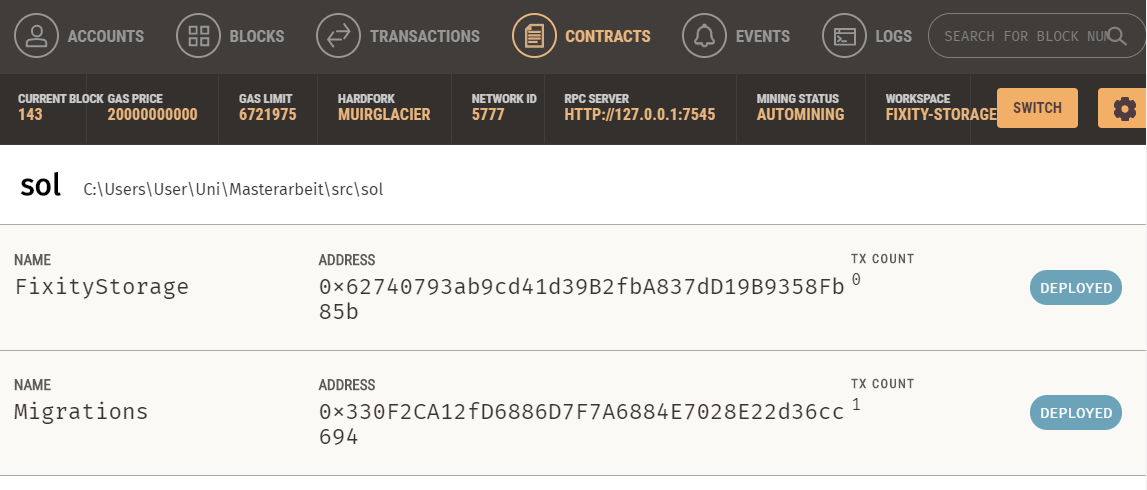
\includegraphics[width=0.7\textwidth]{ganache.png}
\end{figure}
It allows you to click through your smart contract and look at the state variables or functions to validate that your smart contract was successfully deployed. Ganache has a massive disadvantage when doing high throughput computing, it seems that it is not suited to withstand 10000 transactions built in a python for loop. Therefore, I only used the GUI it in the beginning of the experiment where I only persisted about 10 objects at a time without problems. For high throughput computing, truffle offers a command line tool to interact with the blockchain. The command line tool was resistant and showed no weakness when persisting 10000 objects.
Truffle also allows to config other networks, e.g. the Ropsten test network, which can be defined as a parameter in the deployment process. The deployment requires to have some ETH token in your account to pay the miner to integrate your smart contract in a block. 
Truffle offers some utility regarding automated deployment, which are migrations. Migrations are JavaScript files, which are responsible for staging the deployment tasks and running deployment scripts. I used the migrations feature in order to interact with various Ethereum networks, in my case the Ropsten test network and a local test environment. The migrations feature requires to have a smart contract deployed on the blockchain, which causes additional cost (191943 gas) to the fixity storage, therefore I have decided not to use the migrations feature, as it is controversial in the community and seen as unnecessary traffic and cost\footnote{\url{https://github.com/trufflesuite/truffle/issues/503}}.
The deployment cost of the smart contract can be calculated as follows:
\begin{equation}\label{eq:create-cost}
  \begin{split}
      C_{deployment} & = transaction + txcreate + codedeposit + txdatanonzero + txdatazero \\
      & = 21000 + 32000 + 200 * 832 + 226 * 4 + 800 * 16 \\
      & = 233104
  \end{split}
\end{equation}
where $transaction$ is the base cost for a transaction; $txcreate$ is the operation used to create a smart contract; $codedeposit$ is the gas cost for each byte of the runtime bytecode of the smart contract, which is 832 bytes and can be seen in the Input Data field of the transaction on Etherscan\footnote{\url{https://ropsten.etherscan.io/tx/0x844f76cfff6e00f29487f6fe3c99d8a69eab576e7c190e5b392745b48924a1f6}}
\textit{$G_{txdatanonzero}$} is 16 gas for each non-zero byte in the compiled bytecode of a transaction;\textit{$G_{txdatazero}$} is 4 gas for each non-zero byte in the compiled bytecode of a transaction; and \textit{$Contract_{bytesize}$} is the size of the compiled bytecode of the contract, see Section \ref{sec:costs} for the exact gas amount for each transaction.
The amount of gas consumed by the deployment of the decentralized fixity storage is 166079 gas on the Ropsten testnet, the transaction used to deploy the contract can be found on Etherscan\footnote{\url{https://ropsten.etherscan.io/tx/0xf383c4bf0a5c32dd3369b02f68fd4e4400ef59343ad472bc96a28827f32c9abb}}, where additional information can be read. The address of the smart contract is \textit{0x0243c7aa552730E8C6F7ED25A480a7C0c88a70f0}.
\section{Authorized Access}
In solidity one can require a certain address to access a function, the keyword requires can be used  so that a transaction from an unknown address can be reverted and only the owner of the creator address can update the mapped SHA256 values in the smart contract. An interesting topic is also how the private key in the archive may be managed, which is not part of this thesis, but something like a multisignature wallet may be used to split the responsibility of the owner address in the contract. Since the entity which controls the private key of the smart contract is able to perform update operations which can lead to unwanted actions. In the worst case, an unwanted action may be ignored, since the older value is not deleted on the blockchain. Therefore, the key user management of the smart contract can be used as a next step in further research. For this thesis I assume that the private key is well managed and each transaction coming from the master address is legit.
\section{Cost of interacting with the fixity storage}\label{sec:cost-interating}
The cost of interacting with the fixity storage depends on the desired action. There are three different way to interact with the contract: (1) create a new entry (2) update an existing entry and (3) read an entry.
The cost of a transaction, which invokes the setPoolHash function and ultimately stores 256 bit on the blockchain can be calculated with Equation \ref{eq:tx-cost}
\begin{equation}\label{eq:tx-cost}
    \begin{split}
        C_{setPoolHash} & = gasAmount * gasPrice * ethPrice \\ 
        & = 42368 * 0.00000005 * 4000
    \end{split}
\end{equation}
which results in \$8.47 on average for an ETH price of \$4000.
The $gasAmount$ in Equation \ref{eq:tx-cost} can be calculated as follows:
\begin{equation}\label{eq:tx-data}
  \begin{split}
    gasAmount & = transaction + sset + txdatazero + txdatanonzero \\
     & = 21000 + 20000 + 16 * 68 + 4 * 70  \\
     & = 42368
  \end{split}
\end{equation}
where $txdatazero$ is the number of zeros in the transaction data and $txdatanonzero$ is the amount of non-zero bytes in the transaction data. The transaction data for Equation \ref{eq:tx-data} can be found here in the Input Data field of the transaction on Etherscan\footnote{\url{https://ropsten.etherscan.io/tx/0x8839e03f0143bad34060fa909c35d30f2edb22dd4fdac0264de8ae84176eb1ea}}.
The cost for updating an existing entry can be calculated in the same way as for creating ones, with the difference that the costly $sset$ operation can be spared and therefore updates costs 20000 gas less than creates.
Reading an entry is free of charge, since no state changes has to be forwarded to the blockchain.
To explain the cost of the non-zero and zero bytes can be explained by looking the following Input Data

\hash{0x178d292900000000000000000000000000000000000000000000000000000000000000001760d27083f6e2d1c46a65938c03a0c52dccf55cb4eb68a720e6efe3a8851f78}

where zero and nonzero bytes are counted and multiplied by their respective gas cost, which in this example is $txdatazero+txdatanonzero = 4 * 70 + 16 * 68 = 1368 $. The amount of non-zero bytes can be interpreted as the amount of effort given to the network.

\section{Proof of Concept}\label{sec:poc}
The proof of concept is written in Python in form of a Jupyter Notebook. It can be found on GitHub \url{https://github.com/metsch/masterthesis/blob/main/src/py/poc_ropsten.ipynb}. With Python's Web3.py I get the contract from the blockchain and extract its functions setPoolHash and getPoolHash. For the live experiment on the Ropsten test network I have initialized 100 digital objects, in form of SHA256 values, with a prevalence rate of 0.1 (or 10\%). The less amount of objects in the live experiment is due to the fact, that the Ropsten ETH token is hard to get, since the most relevant publicly available faucets are drained out and the ones available have a rate of only 0.1 ETH per day, as I explained in Section \ref{sec:test-nets}. I computed the optimal pool size k for N=100 and p=0.1 with Equation \ref{eq:poolsize} and created $\lceil N/k \rceil$ pools. Each pool is assigned an ID and has an array of objects, from which a hash list is formed, and the resulting root hash is stored. 
Before uploading the pools on to the blockchain, I estimated the gas cost for a single transaction in order to set the gas limit to avoid overpaid transactions. I utilized Equation \ref{eq:tx-data} and added 20\% in order guarantee that the transaction is not underpaid, since the result of Equation \ref{eq:tx-data} is the exact gas amount and may be reverted.
At the time of the experiment, the gas price was 86.11 gwei which is 0,0000000896 ETH, resulting in \$15.18 for a setPoolHash transaction calculated with Equation \ref{eq:tx-cost} with an ETH price of \$4000. Admitted, this gas price is really high, usually the gas price is about 40 gwei. 
For each pool, 25 in total, I uploaded each root hash on to the blockchain and waited for the transaction to finish and run some tests to see if the transactions were successful.
After uploading the root hashes, I artificially corrupted the objects in the archive with a Bernoulli trial where an object gets corrupted if a random number between 0 and 1 is below p=0.1. At last, I repaired the archive by checking the local pools with the ones on the blockchain, and if the pool hashes did match the pool is seen as uncorrupted. Where the pools with non-matching hashes got replaced by copies of the objects.
To sum it up, the cost for the live experiment was for 25 writing transactions 0.11204969029 ETH (\$448) and 8 data-scrubbing operations resulting in 33 total operations. Whereas, with an individual testing strategy the amount of writing transactions would have been 100 and estimated 10 data-scrubbing operations. The experiment showed no weakness in throughput, where 25 transactions were uploaded in an instant and mined in less than 2 minutes

\section{Wrap Up}
In this Chapter I have presented the various forms of fixity information with their respective advantages and disadvantages together with my reasoning on why I have decided to utilize SHA256 cryptographic hashes. I have also presented various storage-media for fixity information and why it is so important that these storages guarantee for immutability in regard to history forgery. The interactions with the fixity storage are tested in an experimental environment, presented in the following section \ref{sec:poc}.
\chapter{Experiment}
\label{ch:experiment}
\section{Setup}
The experiment written in Python in form of a Jupyter Notebook. At first the function for providing the optimal poolsize was implemented, the exact implementation can range froma bernoulli experiment to another form. When the optimal pool sie is found, which is the econd research question I create 10000 objects and assign them to a certain pool and assign them a corruption rate ranging from 0.01 to 0.2. The corruption rate is the base for the bernoulli experiment. After object creation, the objects are ingested into the archive, durng this process each pool is persisted on the blockchain. This happens in an interaction between a python client and a local installation of the ethereum blockchain. Ganache is used for local development on the Ethereum side and pythons Web3 is used as a client. While ingesting and uploading onto the blockchain i will monitor the amount of gas used and the exact number of write transactions. The more eact method of monitoring the operation cost is by adding up the gas cost, since gas can be transformed nto ETH. The first measurement will be theoretical and the second empirical where i monitor the amount of ETH available for the experiment account. e.g. if i start the experiment with 100 ETH and at the end i have 90 ETH left the operation cost was 10 ETH. If the experiment local is successfulll I willl deploy the smart contract on the ropsten testnet and add time measurement to the porcess since the blockchain is now real and distributed on the network. I expect the time needed to ingest and upload on the blockchain to increase the cost should stay the same. When the objects are ingested into thedummy archive and the pools are uploaded onto the blockchain i will retrieve random samples from the original set of objects and check if they are corrupt, maybe i will assign corruption at random to this random sample and then I have to implement a repair function, this ffunction also affect the operation cost, since when a corrupted file is found the whole pool has to be re-computed resulting in poolsize + 1 local transactions and one blockchain write transaction. In the retrieval process i will monitor the time and nullify the cost since read operations on the blockchain are free of charge, nonetheless i will count the number of transactions needed for the process. After retrieval and repairing the pools i will look into the number of transactions needed and the time needed for the whole process. The result will be one row af a table and the experiment can be redone with different poolsies or corruption rates to get a nice table with descriptive statistics. 
At last I will split the objects and metadata and adapt the corruptions rates and redo the whole experiment and compare the results. 
\section{Object Identity}
when and where should the pool id be stored, there are possibilities that the pool id is assigned with pool creation but that would mean that i have to update the object which is supposed to preserve, should the pool id be in the metadata of the object= if no, where should we store the link between the oject and its respective pool. Its easy to keep the links in the local jupyter notebook but in a industrial environment keeiping those links is rather hard. For now i keep the transaction hash with the pool object
\section{Object}
An object in this experiment is simply a SHA256 value, since the preservation process does not care if a picture, text or video is secured by the hash. An object also holds the reference to its pool, where in a real case the poolId is stored in the object's metadata. For the sake of the experiment, the initial bulk is numbered from 1 to N, where the SHA256 value is then assigned to the object. An object also has a float value which indicates the chance of it of being corrupted, this value is used in the bernoulli experiment to determine the optimal pool size based on the corruption rate of all objects. The final member variable of the object is a boolean flag which indicates wheter an object is corrupted or not.

\section{Pool}
A pool in this experiment is a collection of objects with size k. The root hash of a pool is a hash-list of every object in the pool.
\section{Archive Mock}
For the sake of the experiment I will mock the functions of a digital archive in python with the following relevant functions implemented: (1) $bulk_ingest$ (2) retrieve (3) $get_objects_by_poolId$ (4) repair. (1) Is for ingesting a bulk of objects with their respective metadata, it is expected that the poolId is already set for the object. The bulk itself does not know anything about the pool sizes or the amount of pools. The archive therefore is independent of the implementation of a pool and only need to know the poolId of an object. The poolId may be stored in the Preservation Description Information of an object \cite{lee2010open}. (2) Retrieve a single object from the archive. (3) The implementation of this function in a real digital archive may vary from my implementation, where I return every objects stored in the archive with matching poolId. This function is here to provide information regarding the original objects of a pool, this is necessary to rebuild the pool and recalculate the pool hash for someone who might want to check wheter an object in the archive got corrupted. (4) The function which handles the case when a corrupted pool was found. It is a costly function where one write transaction to the blockchain and additional data scrubbing has to be made. When a pool is found to be corrupted, each object in the pool is suspected to be corrupted too and therefore each object has to be replaced by a copy and reassembled in a pool, which hash is then again persisted on the blockchain.
The mock also provides a function to simulate corruption, where each object in the archive has a chance to corrupt itself.
\section{Program Flow}
During development I have seen that the pool size should not be too high.
When a corrupted pool is found, make sure to not double write the same pool to the blockchain
You even got an advantage when you repair objects, since you have do scrub each object in the pool with a fresh copy.
\section{Findings}
in the cleaning process i cant count the reall number of corrupt objects because the number gets diluted by the fact that the local pools are false and even when we get a real object we could not recalculate the pool because the pool itself is corrupted therefore an uncorrupted object is seen here as corrupted since the pool cannot prove it anymore
a positive sideffect is if you find a corrupt elemen you have to scrub the whole pool, which means that the whole pool has is replaced with fresh copies
There are massivele more repairing transactions

\section{Dataset}
I analysed the format-corpus \footnote{\url{https://github.com/openpreserve/format-corpus}} from Open Preserve Foundation \footnote{\url{ http://openpreservation.org/}} to get a better understanding of various file formats, mostly on how volatile they are. The latest commit for my analysis was \textit{commit 4e4b9a34540f72612ba6eab2d28bccceb7a848ae}\footnote{\url{https://github.com/openpreserve/format-corpus/commit/4e4b9a34540f72612ba6eab2d28bccceb7a848ae}} on the 16th of February. The format-corpus is well structured in a public GitHub repo with a decent amount of reputation in form of GitHub stars, where other datasets did provide corrupt links;were not available or did expect a tidious amount of time to download and re-strucutre them. Convenience; diversity of file extensions; and reputation of the organisation affected my decision to use the format-corpus for analysis.
For the analysis I used the python package folderstats\footnote{\url{https://pypi.org/project/folderstats/}} which transforms a directory into a pandas\footnote{\url{https://pandas.pydata.org/}} dataframe. The repository contains 1560 files with 90 distinct file extensions , e.g. 986 \textit{.xml} files which are mostly PRONOM\footnote{\url{https://www.nationalarchives.gov.uk/PRONOM/}} registry files or \textit{pom.xml} files in case of java projects. In Figure \ref{fig:extension_distribution} you can see the distribution of file extensions where \textit{.xml} files make 62.2 percent of the portion and pdf with 6.79 percent as the second largest portion.
\begin{figure}[h]
    \label{fig:extension_distribution}
    \caption{Distribution of file extensions in the format-corpus of Open Preserve Foundation. \url{https://github.com/openpreserve/format-corpus}}
    \centering
    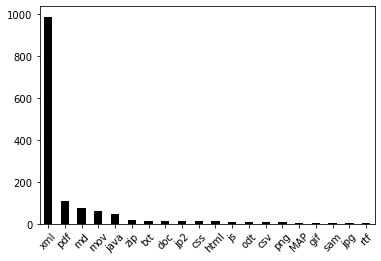
\includegraphics[width=0.5\textwidth]{extension_distribution.png}
\end{figure}
\subsection{Transformations}
To get a baseline estimate on how volatile certain extensions are due to updates and alterations, I analysed Git logs and count how many times a file extension was involved in a commit. The resulting column \textit{positives} was always higher or equal than the occurance of a file extension, since each file was involved in at least one commit, the initial commit of the file. To count the commits I used the python package gitphyton\footnote{\url{https://gitpython.readthedocs.io/en/stable/}} and utilized the git command --log. For each file in the repository, I fired up the command \textit{git log --oneline filename} in python which resulted in one or multiple lines of logs. Latter I used the multiline log as an input for the \textit{.splitlines()} function which results in an array of log lines, the length of this array minus 1 (the initial commit) is used to determine the new column \textit{positives} in the dataframe which shows if and how often a certain file has changed over the lifetime of the git repository. 
This method of determining the volatility of a certain file extension is by no means ideal, but there is no other method to look into how often a certain file has changed without monitoring them on a system for a certain time interval. Therefore I have decided to use the amount of file alterations in the git repository as a rough estimate.
The estimated alteration rate $p$ of a file extension is calculated with $positives/N$, see table \ref{tb:git-alterations}
\begin{table}[ht]
    \caption{Volatility of certain file extensions in the format-corpus dataset}
    \centering
    \begin{tabular}{ c c c c c}
    \label{tb:git-alterations}
     extension & N & positives & p & k\\ 
     \hline
     xml & 986 & 432 & 0.43  & 2\\  
     \hline
     pdf &106 &2 &0.01  & 8\\
     \hline
     md & 74 & 17 & 0.22  & 3\\    
     \hline
     mov&61 & 0 & 0.00 &  61\\  
     \hline
     java &47 &39&0.82 & 2 \\  
     \hline
     zip & 17 &0 &0.00 &  17\\
     \hline
     txt & 14 & 2 & 0.14 &  4\\ 
     \hline
     doc & 13 & 0 & 0.00 &  13\\   
     \hline
     jp2 & 12 & 0 & 0.00 &  12\\    
     \hline
     html & 11 & 6 & 0.54 &  2\\   
     \hline
     css & 11 & 4 & 0.36 & 2 \\ 
     \hline
     js & 10 & 3 & 0.3 & 3
    \end{tabular}
\end{table}
I applied Eq.\ref{eq:simple_poolsize}, created by \cite{regen2020simple}, to each row in Table \ref{tb:git-alterations} to cacluate the optimal poolsize for each file extension.
\begin{equation}\label{eq:simple_poolsize}
    k = 1.24* (positives/N)^-0.466
\end{equation}




\chapter{Evaluation}
\label{ch:evaluation}
The proposed fixity storage is evaluated on a local installation of the Ethereum blockchain and on the online Ropsten test network, where ETH used for transactions are free of charge.
The two key parameters for evaluation are the operation cost and efficiency. 
\textit{Operation cost} is calculated by multiplying the number of relevant cost transactions with the average gas cost of a writing transaction on the blockchain, see Equation \ref{eq:expected_cost}
\begin{equation}\label{eq:expected_cost}
    C = J * C_{setPoolHash} = \lceil N/k \rceil * gasAmount * gasPrice * ethPrice
\end{equation}
where $J$ is the number of pools on ingest; $C_{setPoolHash} $ is the cost for a transaction in gas, see Section \ref{sec:cost-interating}.
I intend to present the operation cost in the form of gas, the unit that measures the amount of computation effort required to execute specific operations, instead of the cost in USD or EUR. This is because, the amount of gas used during the experiment should stay constant, whereas the price of the ETH token fluctuates heavily. Therefore, the amount of gas is a better indicator on how costly the fixity storage is.
\textit{Efficiency} $E(S)$ is measured by the number operations needed utilizing pooled testing compared $T(S_{pooling})$ with the individual testing strategy $T(S_{individual})$, where the efficiency of pooling strategy S is expressed by Equation \ref{eq:efficiency}
\begin{equation}\label{eq:efficiency}
    E(S) = N/T(S)
\end{equation}
where, assuming the preservation process of 10,000 digital objects without pooling requires $N$ operations and the preservation of the same objects using strategy S requires $T(S)$ operations. In the case of individual testing the efficiency is 1, whereas if strategy S requires two times fewer operations the efficiency E(S) is 2 \cite[4]{vzilinskas2021pooled}.

\textit{What is the optimal pool size based on the corruption rates of digital objects in the archive regarding cost and efficiency?}

Corruption rate $p$ represents the prevalence of corruption, e.g., when I assume that 2000 of 10000 objects will be corrupted during the preservation process, $p = 2000/10000 = 0.2$. 

\textit{Expected Operation Cost:} The optimal pool size, which will result in the lowest number of cost relevant transactions is the number of pools $J$, as seen in Equation \ref{fig:expected_cost}, because I only must write onto the blockchain during the ingest process where the root hashes of pools are persisted.
After the first Iteration of the experiment, the number of corrupt objects per positive pools were included in the first draft of Equation \ref{eq:expected_cost}, where I assumed that I had to re-calculate corrupt pool hashes and re-store them on the blockchain, but these "repairing" actions can be done locally through data scrubbing. I only need to know that the pool is corrupt, then I can to substitute each object in the pool with a correct copy in the archive. For this part of the research question, local operations are out of scope because they do not cause direct cost on the blockchain, therefore the optimal pool size calculated by Equation \ref{eq:expected_cost} is $N$, see Figure \ref{fig:expected_cost}. A pool size of $N$ results in exactly 1 cost relevant transaction since I have combined every object on ingest into a hash-list which's root will be stored on the blockchain. This solution does not scale well, e.g., picture the process of retrieving a single object from the archive. In order to guarantee that the object is unaltered, I would have to re-compute the hash list from every object in the archive (or the bulk ingest in question). Additionally, if the single pool is corrupted, I must replace the whole bulk with copies. 
So, there must be an answer, which rewards smaller pool sizes to avoid too much data scrubbing. The number of data scrubbing operations is the number of objects in positive pools on retrieval and is calculated with Equation \ref{eq:expected_data-scrubbing},
\begin{equation}\label{eq:expected_data-scrubbing}
    T(S) = J_+ * k = ((1-(1-p)^k)* \lceil N/k \rceil) * k
\end{equation}
where $(1-p)^k$ is the probability of a pool of size k being negative at a prevalence of p and the probability of a pool being positive is $1-(1-p)^k$. To find the optimal pool size regarding the amount of data scrubbing operations, I had to minimize Equation \ref{eq:expected_data-scrubbing}, as seen in Figure \ref{fig:expected_scrubbing}.
To find the optimal pool size in terms of operation cost and efficiency, operation cost and data scrubbing has to be accounted, which results in the final Equation \ref{eq:expected_operations}
\begin{equation}\label{eq:expected_operations}
    T(S) = J + J_+ * k = \lceil N/k \rceil + ((1-(1-p)^k)* \lceil N/k \rceil) * k
\end{equation}
where \textit{J} is the number of pools and \textit{$J_+ * k$} is the number of objects in corrupted pools. Therefore, the number of expected operations is the number of writing operations on ingest plus the number of data scrubbing operations on retrieval. By adding the amount of data scrubbing operations, the optimal pool size gets significantly lower, see Figure \ref{fig:expected_operations}. The optimal pool size \text{k} can be determined by finding the global minimum of Equation \ref{eq:expected_operations}, which results in the highest efficiency in Equation \ref{eq:efficiency}.
In the experiment, I have utilized Equation \ref{eq:poolsize} presented by \cite[3]{regen2020simple} and round the pool size up in order to avoid non integer pool sizes.
\begin{equation}\label{eq:poolsize}
    k = \lceil 1.24*p^-0.466 \rceil
\end{equation}
\begin{figure}[b]%
    \centering
        \begin{subfigure}{6cm}
        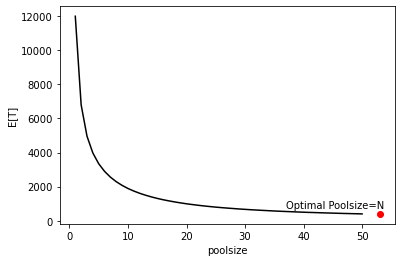
\includegraphics[width=\linewidth]{graphics/expected_cost.png}
        \caption{Optimal pool size regarding the writing transactions. $E[T_w]$}\label{fig:expected_cost}
    \end{subfigure}
    \qquad
    \begin{subfigure}{6cm}
        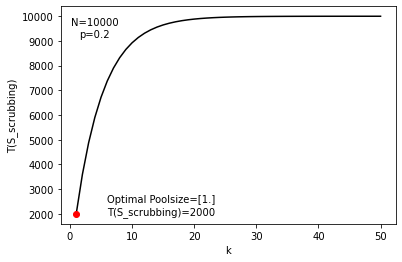
\includegraphics[width=\linewidth]{graphics/expected_scrubbing.png}
        \caption{Optimal pool size regarding the data scrubbing operations $E[T_s]$.}\label{fig:expected_scrubbing}
    \end{subfigure}
    \qquad
    \begin{subfigure}{6cm}
        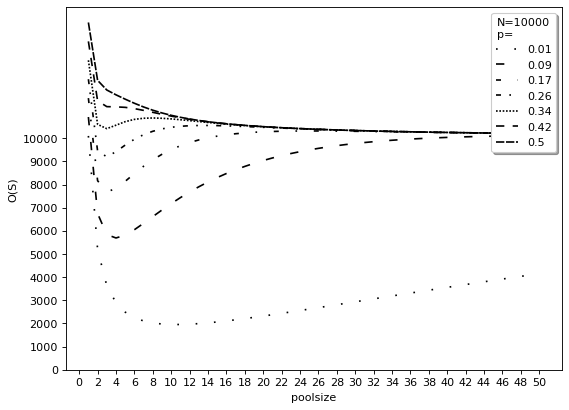
\includegraphics[width=\linewidth]{graphics/expected_operations.png}
        \caption{Optimal pool size regarding the total operations $E[T] = E[T_w]$ + $E[T_s]$.}\label{fig:expected_operations}
    \end{subfigure}
    \caption{Comparison of optimal pool sizes }%
    \label{fig:optimal_pool_size}%
\end{figure}
In Table \ref{tb:expected costs} and Figure \ref{fig:pool-sizes} it is shown that for ingest bulks with higher prevalence of corruption smaller pool sizes are favorable.
\begin{figure}[h]%
    \centering
    \caption{Optimal pool sizes $k$ with prevalence $p$}\label{fig:pool-sizes}
    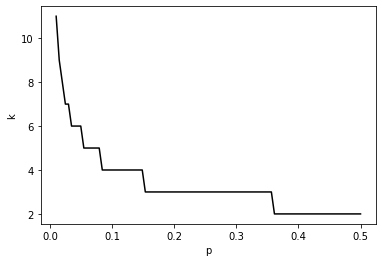
\includegraphics[width=0.5\textwidth]{graphics/poolsizes.png}
\end{figure}
The highest efficiency $E(S)$ can be achieved when the prevalence rate is the lowest, where larger pool sizes are favorable.
\begin{table}[h]
    \caption{Expected transaction throughput with different prevalence of corruption rates}
    \centering
    \begin{tabular}{ c c c c}
    \label{tb:expected costs}
     N & p & k & E(S) \\ 
     10000 & 0.010 & 11 & 5.16 \\ 
     \hline
     10000 & 0.037 & 6 & 2.77 \\  
     \hline
     10000 & 0.065 & 5 & 2.18 \\  
     \hline
     10000 & 0.121 & 4 & 1.71 \\  
     \hline
     10000 & 0.177 & 4 & 1.51  \\
     \hline
     10000 & 0.205 & 3 & 1.45  \\
     \hline
     10000 & 0.316 & 3 & 1.29  \\
     \hline
     10000 & 0.372 & 3 & 1.24  \\
     \hline
     10000 & 0.400 & 2 & 1.22  
    \end{tabular}
\end{table}

\textit{To what extent can pooled testing increase the efficiency and reduce cost for a fixity information storage service on the Ethereum blockchain?}

A context-sensitive approach in the medical field was proposed in 2020 were members of homogeneous groups were pooled, e.g. families, office colleagues or neighbors, and is proven to be more effective than individual testing \cite[4]{deckert2020simulation}. In this thesis, the idea of grouping similar files to increase efficiency of the pooling strategy is implemented by grouping various file extensions, estimating their prevalence in form of alterations and calculating the efficiency per file extension as presented in Equation \ref{eq:efficiency}. The dataset used is presented in Section \ref{sec:dataset}.
\begin{figure}[h]%
    \centering
    \caption{Distribution of prevalence rates $p$}\label{fig:p-distribution}
    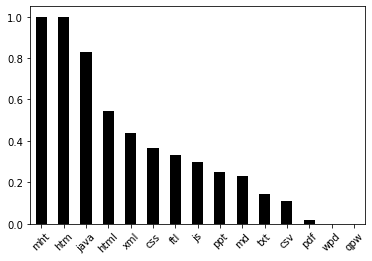
\includegraphics[width=0.5\textwidth]{graphics/p-distribution.png}
\end{figure}
In Figure \ref{fig:p-distribution}, it is shown that the volatility in the repository only affects a few file extensions, where 77 out of 90 file extension where never altered and have therefore a $p$ value of 0.00. These unaltered file extensions are grouped with a group size of $Group_N$, which results in large bulks in the ingest process that have no impact on the retrieval since I assume that no object in this particular group will be altered during the preservation process. For instance, in Table \ref{tb:efficiency}, the file extension MOV has a prevalence rate of $0.00$, and therefore I can assign a group size of $N$ to reach the maximum overall efficiency.
\begin{table}[b]
    \caption{In group efficiency of various file extensions}
    \centering
    \begin{tabular}{ c c c c c c c}
    \label{tb:efficiency}
     extension & N & p & k & T(S) & T($S_{writing}$) & T($S_{scrubbing}$) \\ 
     \hline
     XML & 986 & 0.43 & 2 & 1.21  & 2.00 & 0.64\\  
     \hline
     PDF &106 &0.01 & 8 &  3.60 & 7.57 & 0.12\\
     \hline
     MD & 74 & 0.22  & 3 & 2.96 & 2.00 & 0.41\\    
     \hline
     MOV&61 & 0.00 &  61 & 61.00 & 2.00 & 1.00\\  
     \hline
     JAVA &47 &0.82 & 2  & 1.21 & 1.95 & 0.82\\  
     \hline
     ZIP & 17 &0.00 &  17 & 17.00 & 17.00 & 1.00\\
     \hline
     TXT & 14 & 0.14 &  4 & 1.33 & 3.50 & 0.25\\ 
     \hline
     DOC & 13 & 0.00 &  13 & 13.00 & 13.00 & 1.00\\   
     \hline
     JP2 & 12 & 0.00 &  12 & 12.00 & 12.00 & 1.00\\   
     \hline
     CSS & 11 & 0.36 & 2  & 1.07 & 1.83 & 0.50\\  
     \hline
     HTML & 11 & 0.54 &  2 & 1.06 & 1.83 & 0.60\\   
     \hline
     JS & 10 & 0.3 & 1.08 & 2.50 & 0.50
    \end{tabular}
\end{table}

To calculate the efficiency of the two stage hierarchical pooling strategy, I took the mean $p$ value of the data in Table \ref{tb:efficiency} as an estimator for the overall alteration rate which resulted in 0.06. The input for Equation \ref{eq:expected_operations} was therefore N=1560; p=0.06 and k=5.0.
With context-sensitive pooling, another increase in efficiency can be made. In Table \ref{tb:context-sensitive} I compare the two strategies presented before, with respect to Equation \ref{eq:efficiency}, where the Two-Stage-hierarchical pooling algorithm has achieved an efficiency rate of 2.24 and context-sensitive pooling has achieved an efficiency rate of 3.03. 
\begin{table}[b]
    \caption{Efficiency of context-sensitive pooling vs. two stage hierarchical pooling}
    \centering
    \begin{tabular}{c c}
    \label{tb:context-sensitive}
    Strategy & T(S) \\
    Individual & 1.00 \\
    Two stage hierarchical & 2.24 \\
    Context Sensitive & 3.03 
    \end{tabular}
\end{table}

\textit{RQ 3 Given that metadata has a higher corruption rate, what effect has the split of metadata and objects on the operation cost?}

To know what effect the split off metadata has, I had to double the initial 1560 file extensions and assign the postfix .meta to the newly created rows resulting in Table \ref{tb:metadata},
\begin{table}[b]
    \caption{Arbitrary prevalence rates $p$ and $p_{meta}$ in the format-corpus dataset}
    \centering
    \begin{tabular}{c c c}
    \label{tb:metadata}
    Extension & N & p\\
    METADATA & 1560 & 0.990 \\
    XML& 986 & 0.001 \\
    PDF& 986 & 0.001 \\
    MD& 986 & 0.001 \\
    MOV& 986 & 0.001 
    \end{tabular}
\end{table}
where $p=0.005$ for each file extension and $p_{meta}=0.800$. 
I have calculated the efficiency for context-sensitive and two-stage hierarchical for various combinations of $p$ and $p_{meta}$ and the result is, that with split off metadata the context-sensitive strategy is much worse than the two-stage hierarchical algorithm.
For instance in Table \ref{tb:split-off}, the context-sensitive strategy never even reaches a 1.00 efficiency, which would state that it performs worse as the individual testing in terms of efficiency, whereas the two-stage hierarchical strategy performs better with split off metadata when the $p$ value is low enough. This is because I can assign larger group sizes when the majority of file extensions (the objects) in the dataset do have a very low prevalence rate $p$. This is due to the fact, that the average $p$ value is calculated after grouping the file extensions, where we have only one file extension where the $p$ value is very vast, the metadata.
\begin{table}[b]
    \caption{Arbitrary prevalence rates $p$ and $p_{meta}$ in the format-corpus dataset compared with the individual testing strategy T(N) where 2044 operations are needed.}
    \centering
    \begin{tabular}{c c c c}
    \label{tb:split-off}
    $p$ & $p_{meta}$ & $T(S_{two-stage})$ & $T(S_{context-sensitive})$\\
    0.001 &0.99 & 3.10 & 0.76\\
    0.002 &0.98 & 2.95 & 0.75\\
    0.006 &0.97 & 2.72 & 0.73\\
    0.023 &0.90 & 1.86 & 0.68\\
    0.042 &0.82 & 1.53 & 0.66
    \end{tabular}
\end{table}



\chapter{Discussion}
The first research questions where I did research to find the optimal pool size for the fixity information had two different approaches, the first was to minimize the cost and the second was to maximize the efficiency. The two of them were inversely correlated, where to minimize the cost the pool size was actually N, since there was only one writing transaction on the blockchain when we have only one pool on ingest. On the other hand, a pool size of N is extremely inefficient on retrieval, where I have to replace the whole ingest bulk with fresh copies if only one object in the pool is corrupt, since I cannot determine anymore which object in the pool got corrupted due to the nature of hash lists. Therefore, I had to also account the number of data scrubbing operations into the optimal pool size, resulting in Equation \ref{eq:expected_data-scrubbing}. The pool size is therefore heavily dependent on the prevalence of corruption in the ingest bulk, where if the prevalence is high smaller pool sizes are favorable. The goal of this thesis was to reduce the cost of the fixity storage by at least 50\%, this goal can be met when the optimal pool size is at least two, which is guaranteed with a prevalence lower than 35.9\%, as seen in Figure \ref{fig:threshhold}.
\begin{figure}[h]
    \caption{For a prevalence of corruption of maximum 35.9\%, an optimal pool size of at least two is guaranteed}
    \label{fig:threshhold}
    \centering
    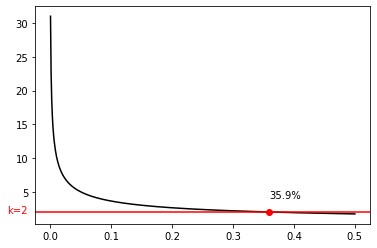
\includegraphics[width=0.5\textwidth]{threshhold.png}
\end{figure}
What happens if the prevalence is higher than 35.9\%, the optimal pool size would be between 1.0 and 2.0 which is not practical since a pool can not include 1.42 objects, therefore I have decided to take the ceil of the result from Equation \ref{eq:poolsize} which results in Figure \ref{fig:threshhold-ceil}.
\begin{figure}[h]
    \caption{For a prevalence of corruption of maximum 35.9\%, an optimal pool size of at least two is guaranteed}
    \label{fig:threshhold-ceil}
    \centering
    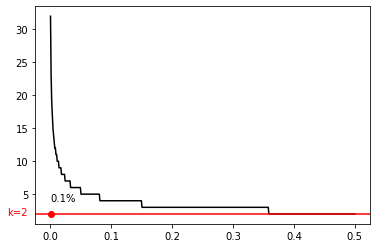
\includegraphics[width=0.5\textwidth]{threshhold-ceil.png}
\end{figure}
For the second research question, I have compared two different approaches for pooled testing. Where the efficiency of both strategies is compared to the efficiency of individual testing. The efficiency of individual testing for sample population of 100 objects where 20 of them are corrupt, meaning that I need 100 writing  + 20 scrubbing operations during the preservation process. With two stage hierarchical pooling an efficiency of 2.24 can be achieved, meaning that this strategy is more than two times as efficient as individual testing. In the format-corpus dataset there were just a few file extensions of 90 that were altered and had a prevalence of corruption greater than 0.0, suggesting that the two-stage strategy was not optimal, since non-volatile files would give been grouped together creating unnecessary traffic on repairing a corrupt pool. Therefore, I have proposed a context-sensitive approach where the inner group prevalence of each file extension is taken into account. Each group in the ingest-bulk is assigned to an own pool with their respective pool size. For instance, in table \ref{tb:efficiency} the file extension PDF has 8 corrupted objects out of 106, which results in a pool size of 8, whereas the XML extension has a much higher corruption rate with an optimal poolside of 2. The context-sensitive approach takes these differences into account and pools homogenous groups, where groups with 0.0 prevalence of corruption can be grouped with a pool size as large as the inner group. With this method, groups with low prevalence can be pooled with large poolside and therefore reduce the cost and increase the efficiency even more than individual testing or two-stage hierarchical pooling.
The third research question had a surprising result, given that metadata has a much higher prevalence of corruption rate than the object themselves, two-stage hierarchical pooling increases its efficiency with split off metadata whereas the context-sensitive strategy looses efficiency by a large margin. This is due, the double amount of objects needed to be processed during the preservation process where the context-sensitive approach can not make up for it, whereas the two-stage hierarchical approach is able to increase the efficiency: due to the low average prevalence of corruption. Because I have N/2 objects with very high prevalence but with the same file extension, therefore we have only one inner group in the dataset with e.g. p=0.99 where the N-1 file extensions have a very low prevalence rate. The imbalance of alteration rates, see Table \ref{tb:context-sensitive}, is favorable because the average prevalence rate gets very low which results in a large pool size in the two-stage approach.
The limitations of the strategies proposed in this thesis is the missing data on prevalence rates on digital objects, this is due to the fact that I would have had to monitor an archive and measure the amount of times an object has changed. In this thesis, I have arbitrarily chosen prevalence rates for the objects and their metadata, see Table \ref{tb:split-off}. Future work may propose a method on how to estimate the prevalence rate of an ingest-bulk in order to calculate the real optimal pool size for the bulk.
The results indicate that the cost for the decentralized fixity storage can be reduced, depending on the prevalence rate of the digital objects by at least 50\%, given that the optimal pool size for an ingest-bulk is at least 2.
\chapter{Conclusion}
While the Ethereum blockchain has its limitation regarding the cost, the results of pooled testing showed in this thesis may include the blockchain in future implementations of fixity information storages. This research has shown that the operation cost can be reduced up to a third of cost, but also raises the question if that is enough to establish the Ethereum blockchain as a storage medium for fixity information due to its high cost. While the security and convenience of the Ethereum blockchain stands out, the cost of persisting fixity information for large ingest bulks in digital archives is still high, even after reducing the cost with pooled testing. Operators of digital archives may consider only persisting the fixity of hand-picked digital objects, where security and availability is needed the most, on the blockchain.

A digital archive could deploy the fixity storage on the Ethereum network by setting up an own Ethereum node or by utilizing the developer tools presented in this thesis. After deployment, the operator of the digital archive would be immediately able to persist fixity information on the blockchain after the installation of an Ethereum client of their choice, such as Pythons Web3.py. Due to its minimal requirements, the proposed solution is lightweight and does not require a larger infrastructure to be executed, since the infrastructure to store the fixity information is provided by the Ethereum blockchain.

The optimal pool size for an ingest bulk is dependent on the change rate of its object. For an ingest of N digital objects, the optimal pool size regarding the operation cost is N. With a pool of size N, you only must write once on the blockchain and therefore minimize the cost. But, for a pooling strategy to be efficient, smaller pool sizes have to be chosen to minimize the number of data-scrubbing operations. Therefore, pool sizes from 2 to 10 are favorable, depending on the change rate of the objects. A pool with size 10 is already at the limit of efficiency and can only be considered for non-volatile digital objects which are not expected to change and may only suffer from bit level errors.

With pooled testing, I was able to reduce the operation cost of preserving the fixity information of 1560 digital objects up to a third. The dataset used is the OpenPreserve format-corpus, an openly licensed dataset consisting of various file set and files from creation tools. The cost, utilizing an individual testing strategy was \$13218.81 whereas with a two-stage-hierarchical approach the cost was \$4406.27. In this thesis, it is also shown that the operation cost in USD is not relevant, since it is heavily dependent on the price of gas and the Ether token, the native cryptocurrency of the Ethereum blockchain. In this thesis, I have chosen to present the operation cost in gas which is a constant value and does not change even when the \acrlong{eth} price rises or falls. The presented amount of gas can be converted into USD or any other currency. I have also shown that the efficiency can be improved by a factor of 1.38 with the implementation of context-sensitive pooling. The context-sensitive approach is slightly more efficient than the two-stage-hierarchical pooling due to its consideration of inner group change rates, whereas two-stage-hierarchical pooling only considers a single change rate over the whole ingest bulk.
The third approach, utilizing split-off metadata has shown to have a worse the cost and efficiency compared to with non-split-off metadata. Although, considering with split-off metadata you have the double number of digital objects, the cost of this approach is still almost halved compared to individual testing.

Future work may include the migration of this proposed fixity information storage to another blockchain, a cheaper one. Although you must consider that the price on the established Ethereum network has its security advantages, e.g., denial-of-service attacks only hurts the attacker because of the cost. A good consideration are so-called Layer 2 solutions, which is a term for Ethereum scaling solutions that handle transactions off Ethereum Layer 1 while still taking advantage of the security\footnote{\url{https://ethereum.org/en/layer-2/}}. Layer 2 solutions are considered faster, cheaper, and therefore would be great candidate to enhance the proposed fixity information storage.\\
Future work may also include the estimation of change rates in ingest-bulks to compute the optimal pool size. In this work, I estimated the change rate of the format-corpus dataset by counting the involvement of certain file extensions in Git commits. My suggestion for the estimation is to monitor a digital archive for a certain time interval and count the number of times a certain object has changed. Another interesting method would be, to estimate the change rate of an object based on its file size. If a larger file has a higher chance to experience a bit level error during long term storage.

My contribution to archival science and preservation research was to gather the exact computational effort, in form of gas, needed to operate a decentralized fixity information storage on the Ethereum blockchain. Additionally, I have presented a method to decrease the number of operations and therefore the number of cost relevant transactions needed to operate such an application. With pooled testing, the operation cost of storing the fixity information for 1560 files in format-corpus dataset has been reduced to a third of the cost.




% Remove following line for the final thesis.
%%% intro.tex
%% Copyright (C) 2014-2020 by Thomas Auzinger <thomas@auzinger.name>
%
% This work may be distributed and/or modified under the
% conditions of the LaTeX Project Public License, either version 1.3
% of this license or (at your option) any later version.
% The latest version of this license is in
%   http://www.latex-project.org/lppl.txt
% and version 1.3 or later is part of all distributions of LaTeX
% version 2005/12/01 or later.
%
% This work has the LPPL maintenance status `maintained'.
%
% The Current Maintainer of this work is Thomas Auzinger.
%
% This work consists of the files vutinfth.dtx and vutinfth.ins
% and the derived file vutinfth.cls.
% This work also consists of the file intro.tex.


\newacronym{ctan}{CTAN}{Comprehensive TeX Archive Network}
\newacronym{faq}{FAQ}{Frequently Asked Questions}
\newacronym{pdf}{PDF}{Portable Document Format}
\newacronym{svn}{SVN}{Subversion}
\newacronym{wysiwyg}{WYSIWYG}{What You See Is What You Get}

\newglossaryentry{texteditor}
{
  name={editor},
  description={A text editor is a type of program used for editing plain text files.}
}

\chapter{Introduction to \LaTeX}

Since \LaTeX\ is widely used in academia and industry, there exists a plethora of freely accessible introductions to the language.
Reading through the guide at \url{https://en.wikibooks.org/wiki/LaTeX} serves as a comprehensive overview for most of the functionality and is highly recommended before starting with a thesis in \LaTeX.

\section{Installation}

A full \LaTeX\ distribution\index{distribution} consists not only of the binaries that convert the source files to the typeset documents, but also of a wide range of packages and their documentation.
Depending on the operating system, different implementations are available as shown in Table~\ref{tab:distrib}.
\textbf{Due to the large amount of packages that are in everyday use and due to their high interdependence, it is paramount to keep the installed distribution\index{distribution} up to date.}
Otherwise, obscure errors and tedious debugging ensue.

\begin{table}
  \centering
  \begin{tabular}{cccc}
    \toprule
    Distribution & Unix         & Windows      & MacOS        \\
    \midrule
    TeX Live     & \textbf{yes} & yes          & (yes)        \\
    MacTeX       & no           & no           & \textbf{yes} \\
    MikTeX       & (yes)        & \textbf{yes} & yes          \\
    \bottomrule
  \end{tabular}
  \caption{\TeX/\LaTeX\ distributions for different operating systems. Recomended choice in \textbf{bold}.}
  \label{tab:distrib} % \label has to be placed AFTER \caption to produce correct cross-references.
\end{table}

\section{Editors}

A multitude of \TeX\ \glspl{texteditor} are available differing in their editing models, their supported operating systems and their feature sets.
A comprehensive overview of \glspl{texteditor} can be found at the Wikipedia page  \url{https://en.wikipedia.org/wiki/Comparison_of_TeX_editors}.
TeXstudio (\url{http://texstudio.sourceforge.net/}) is recommended.
Most editors support a synchronization of the generated document and the \LaTeX\ source by \verb|Ctrl| clicking either on the source document or the generated document.

\section{Compilation}

Modern editors usually provide the compilation programs to generate \gls{pdf} documents and for most \LaTeX\ source files, this is sufficient.
More advanced \LaTeX\ functionality, such as glossaries and bibliographies, needs additional compilation steps, however.
It is also possible that errors in the compilation process invalidate intermediate files and force subsequent compilation runs to fail.
It is advisable to delete intermediate files (\verb|.aux|, \verb|.bbl|, etc.), if errors occur and persist.
All files that are not generated by the user are automatically regenerated.
To compile the current document, the steps as shown in Table~\ref{tab:compile} have to be taken.


\begin{table}
  \centering
  \begin{tabular}{rl}
    \toprule
    & Description \\
    \midrule
    1 & Scan for refs, toc/lof/lot/loa items and cites \\
    2 & Build the bibliography     \\
    3 & Link refs and build the toc/lof/lot/loa \\
    4 & Link the bibliography \\
    5 & Build the glossary \\
    6 & Build the acronyms \\
    7 & Build the index \\
    8 & Link the glossary, acronyms, and the index \\
    9 & Link the bookmarks \\
    \midrule
    & Command \\
    \midrule
    1 & \verb|pdflatex.exe  example| \\
    2 & \verb|bibtex.exe    example| \\
    3 & \verb|pdflatex.exe  example| \\
    4 & \verb|pdflatex.exe  example| \\
    5 & \verb|makeindex.exe -t example.glg -s example.ist| \\
      & \verb|              -o example.gls example.glo| \\
    6 & \verb|makeindex.exe -t example.alg -s example.ist| \\
      & \verb|              -o example.acr example.acn| \\
    7 & \verb|makeindex.exe -t example.ilg -o example.ind example.idx| \\
    8 & \verb|pdflatex.exe  example| \\
    9 & \verb|pdflatex.exe  example| \\
    \bottomrule
  \end{tabular}
  \caption{Compilation steps for this document. The following abbreviations were used: table of contents (toc), list of figures (lof), list of tables (lot), list of algorithms (loa).}
  \label{tab:compile} % \label has to be placed AFTER \caption to produce correct cross-references.
\end{table}


\section{Basic Functionality}

In this section, various examples are given of the fundamental building blocks used in a thesis.
Many \LaTeX\ commands have a rich set of options that can be supplied as optional arguments.
The documentation of each command should be consulted to get an impression of the full spectrum of its functionality.

\subsection{Floats}

Two main categories of page elements can be differentiated in the usual \LaTeX\ workflow: \textit{(i)} the main stream of text and \textit{(ii)} floating containers that are positioned at convenient positions throughout the document.
In most cases, tables, plots, and images are put into such containers since they are usually positioned at the top or bottom of pages.
These are realized by the two environments \verb|figure| and \verb|table|, which also provide functionality for cross-referencing (see Table~\ref{tab:intro} and Figure~\ref{fig:intro}) and the generation of corresponding entries in the list of figures and the list of tables.
Note that these environments solely act as containers and can be assigned arbitrary content.

\subsection{Tables}

A table in \LaTeX\ is created by using a \verb|tabular| environment or any of its extensions, e.g., \verb|tabularx|.
The commands \verb|\multirow| and \verb|\multicolumn| allow table elements to span multiple rows and columns.

\begin{table}[h] % placement specifier
  \centering
  \begin{tabular}{lll}
    \toprule
    \multicolumn{2}{c}{Position} \\
    \cmidrule{1-2} % partial horizontal rule
    Group & Abbrev & Name \\
    \midrule
    Goalkeeper & GK & Paul Robinson \\
    \midrule
    \multirow{4}{*}{Defenders} & LB & Lucus Radebe \\
                               & DC & Michael Duburry \\
                               & DC & Dominic Matteo \\
                               & RB & Didier Domi \\
    \midrule
    \multirow{3}{*}{Midfielders} & MC & David Batty \\
                                 & MC & Eirik Bakke \\
                                 & MC & Jody Morris \\
    \midrule
    Forward & FW & Jamie McMaster \\
    \midrule
    \multirow{2}{*}{Strikers} & ST & Alan Smith \\
                              & ST & Mark Viduka \\
    \bottomrule
  \end{tabular}
  \caption{Adapted example from the \LaTeX guide at \url{https://en.wikibooks.org/wiki/LaTeX/Tables}. This example uses rules specific to the \texttt{booktabs} package and employs the multi-row functionality of the \texttt{multirow} package.}
  \label{tab:intro} % \label has to be placed AFTER \caption to produce correct cross-references.
\end{table}

\subsection{Images}

An image is added to a document via the \verb|\includegraphics| command as shown in Figure~\ref{fig:intro}.
The \verb|\subcaption| command can be used to reference subfigures, such as Figure~\ref{fig:intro:full width} and~\ref{fig:intro:half width}.

\begin{figure}[h]
  \centering
  \begin{subfigure}[b]{0.45\columnwidth}
    \centering
    
\includegraphics[width=\textwidth]{Logo-schwarz.pdf}
    \subcaption{The header logo at text width.}
    \label{fig:intro:full width}
  \end{subfigure}
  \begin{subfigure}[b]{0.45\columnwidth}
    \centering
    
\includegraphics[width=0.5\textwidth]{Logo-schwarz.pdf}
    \subcaption{The header logo at half the text width.}
    \label{fig:intro:half width}
  \end{subfigure}
  \caption[Optional caption for the figure list (often used to abbreviate long captions)]{The header logo at different sizes.} % Remove the [...] argument if the original caption should be used in the figure list.
  \label{fig:intro} % \label has to be placed AFTER \caption (or \subcaption) to produce correct cross-references.
\end{figure}

\subsection{Mathematical Expressions}

One of the original motivation to create the \TeX\ system was the need for mathematical typesetting.
To this day, \LaTeX\ is the preferred system to write math-heavy documents and a wide variety of functions aids the author in this task.
A mathematical expression can be inserted inline as $\sum_{n=1}^{\infty} \frac{1}{n^2} = \frac{\pi^2}{6}$ outside of the text stream as \[ \sum_{n=1}^{\infty} \frac{1}{n^2} = \frac{\pi^2}{6} \] or as numbered equation with
\begin{equation}
\sum_{n=1}^{\infty} \frac{1}{n^2} = \frac{\pi^2}{6}.
\end{equation}

\subsection{Pseudo Code}

The presentation of algorithms can be achieved with various packages; the most popular are \verb|algorithmic|, \verb|algorithm2e|, \verb|algorithmicx|, or \verb|algpseudocode|.
An overview is given at \url{https://tex.stackexchange.com/questions/229355}.
An example of the use of the \verb|alogrithm2e| package is given with Algorithm~\ref{alg:gauss-seidel}.

\begin{algorithm}
  \SetKw{BreakFor}{break for}
  \KwIn{A scalar~$\epsilon$, a matrix $\mathbf{A} = (a_{ij})$, a vector $\vec{b}$, and an initial vector $\vec{x}^{(0)}$}
  \KwOut{$\vec{x}^{(n)}$ with $\mathbf{A} \vec{x}^{(n)} \approx \vec{b}$}
  \For{$k\leftarrow 1$ \KwTo maximum iterations}
  {
     \For{$i\leftarrow 1$ \KwTo $n$}
     {
        $x_i^{(k)} = \frac{1}{a_{ii}} \left(b_i-\sum_{j<i} a_{ij} x_j^{(k)} - \sum_{j>i} a_{ij} x_j^{(k-1)} \right)$\;
     }
     \If{$\lvert\vec{x}^{(k)}-\vec{x}^{(k-1)}\rvert < \epsilon$}
     {\BreakFor\;}
  }
  \Return{$\vec{x}^{(k)}$\;}
  \caption{Gauss-Seidel}
  \label{alg:gauss-seidel} % \label has to be placed AFTER \caption to produce correct cross-references.
\end{algorithm}

\section{Bibliography}

The referencing of prior work is a fundamental requirement of academic writing and well supported by \LaTeX.
The \textsc{Bib}\TeX\ reference management software is the most commonly used system for this purpose.
Using the \verb|\cite| command, it is possible to reference entries in a \verb|.bib| file out of the text stream, e.g., as~\cite{Turing1936}.
The generation of the formatted bibliography needs a separate execution of \verb|bibtex.exe| (see Table~\ref{tab:compile}).

\section{Table of Contents}

The table of contents is automatically built by successive runs of the compilation, e.g., of \verb|pdflatex.exe|.
The command \verb|\setsecnumdepth| allows the specification of the depth of the table of contents and additional entries can be added to the table of contents using \verb|\addcontentsline|.
The starred versions of the sectioning commands, i.e., \verb|\chapter*|, \verb|\section*|, etc., remove the corresponding entry from the table of contents.

\section{Acronyms / Glossary / Index}

The list of acronyms, the glossary, and the index need to be built with a separate execution of \verb|makeindex| (see Table~\ref{tab:compile}).
Acronyms have to be specified with \verb|\newacronym| while glossary entries use \verb|\newglossaryentry|.
Both are then used in the document content with one of the variants of \verb|\gls|, such as \verb|\Gls|, \verb|\glspl|, or \verb|\Glspl|.
Index items are simply generated by placing \verb|\index|\marg{entry} next to all the words that correspond to the index entry \meta{entry}.
Note that many enhancements exist for these functionalities and the documentation of the \verb|makeindex| and the \verb|glossaries| packages should be consulted.

\section{Tips}

Since \TeX\ and its successors do not employ a \gls{wysiwyg} editing scheme, several guidelines improve the readability of the source content:
\begin{itemize}
\item Each sentence in the source text should start with a new line.
      This helps not only the user navigation through the text, but also enables revision control systems (e.g. \gls{svn}, Git) to show the exact changes authored by different users.
      Paragraphs are separated by one (or more) empty lines.
\item Environments, which are defined by a matching pair of \verb|\begin{name}| and \verb|\end{name}|, can be indented by whitespace to show their hierarchical structure.
\item In most cases, the explicit use of whitespace (e.g. by adding \verb|\hspace{4em}| or \verb|\vspace{1.5cm}|) violates typographic guidelines and rules.
      Explicit formatting should only be employed as a last resort and, most likely, better ways to achieve the desired layout can be found by a quick web search.
\item The use of bold or italic text is generally not supported by typographic considerations and the semantically meaningful \verb|\emph{|\texttt{$\dots$}\verb|}| should be used.
\end{itemize}

The predominant application of the \LaTeX\ system is the generation of \gls{pdf} files via the \textsc{Pdf}\LaTeX\ binaries.
In the current version of \textsc{Pdf}\LaTeX, it is possible that absolute file paths and user account names are embedded in the final \gls{pdf} document.
While this poses only a minor security issue for all documents, it is highly problematic for double blind reviews.
The process shown in Table~\ref{tab:ps2pdf} can be employed to strip all private information from the final \gls{pdf} document.

\begin{table}[h]
  \centering
  \begin{tabular}{rl}
  \toprule
  & Command \\
  \midrule
  1 & Rename the \gls{pdf} document \verb|final.pdf| to \verb|final.ps|. \\
  2 & Execute the following command: \\
    & \verb|ps2pdf -dPDFSETTINGS#/prepress ^| \\
    & \verb| -dCompatibilityLevel#1.4 ^| \\
    & \verb| -dAutoFilterColorImages#false ^| \\
    & \verb| -dAutoFilterGrayImages#false ^| \\
    & \verb| -dColorImageFilter#/FlateEncode ^| \\
    & \verb| -dGrayImageFilter#/FlateEncode ^| \\
    & \verb| -dMonoImageFilter#/FlateEncode ^| \\
    & \verb| -dDownsampleColorImages#false ^| \\
    & \verb| -dDownsampleGrayImages#false ^| \\
    & \verb| final.ps final.pdf| \\
  \bottomrule
  \end{tabular}

  On Unix-based systems, replace \verb|#| with \verb|=| and \verb|^| with \verb|\|.
  \caption{Anonymization of \gls{pdf} documents.}
  \label{tab:ps2pdf}
\end{table}

\section{Resources}

\subsection{Useful Links}

In the following, a listing of useful web resources is given.
\begin{description}
\item[\url{https://en.wikibooks.org/wiki/LaTeX}] An extensive wiki-based guide to \LaTeX.
\item[\url{http://www.tex.ac.uk/faq}] A (huge) set of \gls{faq} about \TeX\ and \LaTeX.
\item[\url{https://tex.stackexchange.com/}] The definitive user forum for non-trivial \LaTeX-related questions and answers.
\end{description}

\subsection[Comprehensive TeX Archive Network]{\gls{ctan}}

The \gls{ctan} is the official repository for all \TeX\ related material.
It can be accessed via \url{https://www.ctan.org/} and hosts (among other things) a huge variety of packages that provide extended functionality for \TeX\ and its successors.
Note that most packages contain \gls{pdf} documentation that can be directly accessed via \gls{ctan}.

In the following, a short, non-exhaustive list of relevant \gls{ctan}-hosted packages is given together with their relative path.
\begin{description}[itemsep=0ex]
\item[\href{https://www.ctan.org/pkg/algorithm2e}{algorithm2e}] Functionality for writing pseudo code.
\item[\href{https://www.ctan.org/pkg/amsmath}{amsmath}] Enhanced functionality for typesetting mathematical expressions.
\item[\href{https://www.ctan.org/pkg/amsfonts}{amssymb}] Provides a multitude of mathematical symbols.
\item[\href{https://www.ctan.org/pkg/booktabs}{booktabs}] Improved typesetting of tables.
\item[\href{https://www.ctan.org/pkg/enumitem}{enumitem}] Control over the layout of lists (\verb|itemize|, \verb|enumerate|, \verb|description|).
\item[\href{https://www.ctan.org/pkg/fontenc}{fontenc}] Determines font encoding of the output.
\item[\href{https://www.ctan.org/pkg/glossaries}{glossaries}] Create glossaries and list of acronyms.
\item[\href{https://www.ctan.org/pkg/graphicx}{graphicx}] Insert images into the document.
\item[\href{https://www.ctan.org/pkg/inputenc}{inputenc}] Determines encoding of the input.
\item[\href{https://www.ctan.org/pkg/l2tabu}{l2tabu}] A description of bad practices when using \LaTeX.
\item[\href{https://www.ctan.org/pkg/mathtools}{mathtools}] Further extension of mathematical typesetting.
\item[\href{https://www.ctan.org/pkg/memoir}{memoir}] The document class on upon which the \verb|vutinfth| document class is based.
\item[\href{https://www.ctan.org/pkg/multirow}{multirow}] Allows table elements to span several rows.
\item[\href{https://www.ctan.org/pkg/pgfplots}{pgfplots}] Function plot drawings.
\item[\href{https://www.ctan.org/pkg/pgf}{pgf/TikZ}] Creating graphics inside \LaTeX\ documents.
\item[\href{https://www.ctan.org/pkg/subcaption}{subcaption}] Allows the use of subfigures and enables their referencing.
\item[\href{https://www.ctan.org/tex-archive/info/symbols/comprehensive/}{symbols/comprehensive}] A listing of around 5000 symbols that can be used with \LaTeX.
\item[\href{https://www.ctan.org/pkg/voss-mathmode}{voss-mathmode}] A comprehensive overview of typesetting mathematics in \LaTeX.
\item[\href{https://www.ctan.org/pkg/xcolor}{xcolor}] Allows the definition and use of colors.
\end{description} % A short introduction to LaTeX.

\backmatter

% Use an optional list of figures.
%\listoffigures % Starred version, i.e., \listoffigures*, removes the toc entry.

% Use an optional list of tables.
%\cleardoublepage % Start list of tables on the next empty right hand page.
%\listoftables % Starred version, i.e., \listoftables*, removes the toc entry.

% Use an optional list of alogrithms.
%\listofalgorithms
%\addcontentsline{toc}{chapter}{List of Algorithms}

% Add an index.
\printindex

% Add a glossary.
\printglossaries

% Add a bibliography.
\bibliographystyle{alpha}
\bibliography{bibliography}
\todo{Enter your text here.}
\end{document}